% Options for packages loaded elsewhere
\PassOptionsToPackage{unicode}{hyperref}
\PassOptionsToPackage{hyphens}{url}
%
\documentclass[
]{article}
\usepackage{lmodern}
\usepackage{amssymb,amsmath}
\usepackage{ifxetex,ifluatex}
\ifnum 0\ifxetex 1\fi\ifluatex 1\fi=0 % if pdftex
  \usepackage[T1]{fontenc}
  \usepackage[utf8]{inputenc}
  \usepackage{textcomp} % provide euro and other symbols
\else % if luatex or xetex
  \usepackage{unicode-math}
  \defaultfontfeatures{Scale=MatchLowercase}
  \defaultfontfeatures[\rmfamily]{Ligatures=TeX,Scale=1}
\fi
% Use upquote if available, for straight quotes in verbatim environments
\IfFileExists{upquote.sty}{\usepackage{upquote}}{}
\IfFileExists{microtype.sty}{% use microtype if available
  \usepackage[]{microtype}
  \UseMicrotypeSet[protrusion]{basicmath} % disable protrusion for tt fonts
}{}
\makeatletter
\@ifundefined{KOMAClassName}{% if non-KOMA class
  \IfFileExists{parskip.sty}{%
    \usepackage{parskip}
  }{% else
    \setlength{\parindent}{0pt}
    \setlength{\parskip}{6pt plus 2pt minus 1pt}}
}{% if KOMA class
  \KOMAoptions{parskip=half}}
\makeatother
\usepackage{xcolor}
\IfFileExists{xurl.sty}{\usepackage{xurl}}{} % add URL line breaks if available
\IfFileExists{bookmark.sty}{\usepackage{bookmark}}{\usepackage{hyperref}}
\hypersetup{
  pdftitle={Bank Loan Classification - HarvardX Capstone Project},
  pdfauthor={Pradeep Kumar},
  hidelinks,
  pdfcreator={LaTeX via pandoc}}
\urlstyle{same} % disable monospaced font for URLs
\usepackage[margin=1in]{geometry}
\usepackage{color}
\usepackage{fancyvrb}
\newcommand{\VerbBar}{|}
\newcommand{\VERB}{\Verb[commandchars=\\\{\}]}
\DefineVerbatimEnvironment{Highlighting}{Verbatim}{commandchars=\\\{\}}
% Add ',fontsize=\small' for more characters per line
\usepackage{framed}
\definecolor{shadecolor}{RGB}{42,33,28}
\newenvironment{Shaded}{\begin{snugshade}}{\end{snugshade}}
\newcommand{\AlertTok}[1]{\textcolor[rgb]{1.00,1.00,0.00}{#1}}
\newcommand{\AnnotationTok}[1]{\textcolor[rgb]{0.00,0.40,1.00}{\textbf{\textit{#1}}}}
\newcommand{\AttributeTok}[1]{\textcolor[rgb]{0.74,0.68,0.62}{#1}}
\newcommand{\BaseNTok}[1]{\textcolor[rgb]{0.27,0.67,0.26}{#1}}
\newcommand{\BuiltInTok}[1]{\textcolor[rgb]{0.74,0.68,0.62}{#1}}
\newcommand{\CharTok}[1]{\textcolor[rgb]{0.02,0.61,0.04}{#1}}
\newcommand{\CommentTok}[1]{\textcolor[rgb]{0.00,0.40,1.00}{\textbf{\textit{#1}}}}
\newcommand{\CommentVarTok}[1]{\textcolor[rgb]{0.74,0.68,0.62}{#1}}
\newcommand{\ConstantTok}[1]{\textcolor[rgb]{0.74,0.68,0.62}{#1}}
\newcommand{\ControlFlowTok}[1]{\textcolor[rgb]{0.26,0.66,0.93}{\textbf{#1}}}
\newcommand{\DataTypeTok}[1]{\textcolor[rgb]{0.74,0.68,0.62}{\underline{#1}}}
\newcommand{\DecValTok}[1]{\textcolor[rgb]{0.27,0.67,0.26}{#1}}
\newcommand{\DocumentationTok}[1]{\textcolor[rgb]{0.00,0.40,1.00}{\textit{#1}}}
\newcommand{\ErrorTok}[1]{\textcolor[rgb]{1.00,1.00,0.00}{\textbf{#1}}}
\newcommand{\ExtensionTok}[1]{\textcolor[rgb]{0.74,0.68,0.62}{#1}}
\newcommand{\FloatTok}[1]{\textcolor[rgb]{0.27,0.67,0.26}{#1}}
\newcommand{\FunctionTok}[1]{\textcolor[rgb]{1.00,0.58,0.35}{\textbf{#1}}}
\newcommand{\ImportTok}[1]{\textcolor[rgb]{0.74,0.68,0.62}{#1}}
\newcommand{\InformationTok}[1]{\textcolor[rgb]{0.00,0.40,1.00}{\textbf{\textit{#1}}}}
\newcommand{\KeywordTok}[1]{\textcolor[rgb]{0.26,0.66,0.93}{\textbf{#1}}}
\newcommand{\NormalTok}[1]{\textcolor[rgb]{0.74,0.68,0.62}{#1}}
\newcommand{\OperatorTok}[1]{\textcolor[rgb]{0.74,0.68,0.62}{#1}}
\newcommand{\OtherTok}[1]{\textcolor[rgb]{0.74,0.68,0.62}{#1}}
\newcommand{\PreprocessorTok}[1]{\textcolor[rgb]{0.74,0.68,0.62}{\textbf{#1}}}
\newcommand{\RegionMarkerTok}[1]{\textcolor[rgb]{0.74,0.68,0.62}{#1}}
\newcommand{\SpecialCharTok}[1]{\textcolor[rgb]{0.02,0.61,0.04}{#1}}
\newcommand{\SpecialStringTok}[1]{\textcolor[rgb]{0.02,0.61,0.04}{#1}}
\newcommand{\StringTok}[1]{\textcolor[rgb]{0.02,0.61,0.04}{#1}}
\newcommand{\VariableTok}[1]{\textcolor[rgb]{0.74,0.68,0.62}{#1}}
\newcommand{\VerbatimStringTok}[1]{\textcolor[rgb]{0.02,0.61,0.04}{#1}}
\newcommand{\WarningTok}[1]{\textcolor[rgb]{1.00,1.00,0.00}{\textbf{#1}}}
\usepackage{longtable,booktabs}
% Correct order of tables after \paragraph or \subparagraph
\usepackage{etoolbox}
\makeatletter
\patchcmd\longtable{\par}{\if@noskipsec\mbox{}\fi\par}{}{}
\makeatother
% Allow footnotes in longtable head/foot
\IfFileExists{footnotehyper.sty}{\usepackage{footnotehyper}}{\usepackage{footnote}}
\makesavenoteenv{longtable}
\usepackage{graphicx,grffile}
\makeatletter
\def\maxwidth{\ifdim\Gin@nat@width>\linewidth\linewidth\else\Gin@nat@width\fi}
\def\maxheight{\ifdim\Gin@nat@height>\textheight\textheight\else\Gin@nat@height\fi}
\makeatother
% Scale images if necessary, so that they will not overflow the page
% margins by default, and it is still possible to overwrite the defaults
% using explicit options in \includegraphics[width, height, ...]{}
\setkeys{Gin}{width=\maxwidth,height=\maxheight,keepaspectratio}
% Set default figure placement to htbp
\makeatletter
\def\fps@figure{htbp}
\makeatother
\setlength{\emergencystretch}{3em} % prevent overfull lines
\providecommand{\tightlist}{%
  \setlength{\itemsep}{0pt}\setlength{\parskip}{0pt}}
\setcounter{secnumdepth}{5}

\title{Bank Loan Classification - HarvardX Capstone Project}
\author{Pradeep Kumar}
\date{19/06/2020}

\begin{document}
\maketitle

{
\setcounter{tocdepth}{2}
\tableofcontents
}
\hypertarget{executive-summary}{%
\section{Executive Summary}\label{executive-summary}}

As part of its customer acquisition efforts, \textbf{Bank of India}
wants to run a campaign to convince more of its current customers to
accept personal loan offers. In order to improve targeting quality, they
want to find customers that are most likely to accept the personal loan
offer. The dataset is from a previous campaign on 5,000 customers, 4,80
of them accepted. The metrics used to evaluate the models is
\textbf{Classification Accuracy and F1-Score}; Although Accuracy is
useful, we consider the F1-Score because the prediction class is
unbalanced.\\
We have obtained an \textbf{F1-Score} of approximately \textbf{0.911}
and Accuracy of \textbf{98.31\%} for the best performing model.

\pagebreak

\hypertarget{introduction}{%
\section{Introduction}\label{introduction}}

We use the dataset to solve the classification task. We go through the
machine learning pipeline, starting with reading the dataset and
exploring the data through plots and summaries. Then, we move to
preprocess the data to standardize the data and check for any missing
values. Later, we build models to classify the data. Finally, we
evaluate the best models using the whole test dataset.

\hypertarget{objective-of-the-project}{%
\subsection{Objective of the project}\label{objective-of-the-project}}

The goal of this project is to train a machine learning model that
classifies whether or not a customer will take a personal loan. Hence,
the target variable is \textbf{Personal Loan}.

The metric used to evaluate the model's performance is the F1-Score. It
is used because we have an unbalanced dataset. It tries to maximize both
precision and recall.

\hypertarget{dataset}{%
\subsection{Dataset}\label{dataset}}

The dataset used is the
\href{https://datasetbankofindia.s3.ap-south-1.amazonaws.com/Bank_of_India.csv}{Bank
of India dataset} of 5,000 customers.\\
The dataset is from a previous campaign on 5,000 customers run by the
bank.

The \textbf{variables in the dataset} are described as follows:

\begin{verbatim}
1. id: Customer ID
2. age: Customer's age in completed years
3. experience: Number of years of professional experience
4. income: Annual income of the customer (in thousands)
5. zip: Home Address ZIP code.
6. family: The family size of the customer
7. credit_card_spend: Avg. spending on credit cards per month (in thousands)
8. education: Education Level. 1: Undergrad; 2: Graduate; 3: Advanced/Professional
9. mortgage: Value of house mortgage if any. (in thousands)
10. personal_loan: Did this customer accept the personal loan offered in the last campaign?
11. securities_account: Does the customer have securities account with the bank?
12. cd_account: Does the customer have a certificate of deposit (CD) account with the bank?
13. online: Does the customer use internet banking facilities?
14. credit_card: Does the customer use a credit card issued by Bank?
\end{verbatim}

We read the dataset using either the local file, if available offline,
or directly from the set up amazon s3 bucket.

\begin{Shaded}
\begin{Highlighting}[]
\CommentTok{# Read data directly from my s3 bucket}
\NormalTok{raw_data<-}\KeywordTok{read_csv}\NormalTok{(}\StringTok{"https://datasetbankofindia.s3.ap-south-1.amazonaws.com/Bank_of_India.csv"}\NormalTok{)}

\CommentTok{# Read data from local file if you clone my repo}
\CommentTok{# raw_data <- read_csv("./dataset/Bank_of_India.csv")}
\end{Highlighting}
\end{Shaded}

First, To get familiar with the dataset, we look at the head of the
dataset.

\begin{verbatim}
## # A tibble: 6 x 14
##      id   age experience income   zip family credit_card_spe~ education mortgage
##   <dbl> <dbl>      <dbl>  <dbl> <dbl>  <dbl>            <dbl>     <dbl>    <dbl>
## 1     1    25          1     49 91107      4              1.6         1        0
## 2     2    45         19     34 90089      3              1.5         1        0
## 3     3    39         15     11 94720      1              1           1        0
## 4     4    35          9    100 94112      1              2.7         2        0
## 5     5    35          8     45 91330      4              1           2        0
## 6     6    37         13     29 92121      4              0.4         2      155
## # ... with 5 more variables: personal_loan <dbl>, securities_account <dbl>,
## #   cd_account <dbl>, online <dbl>, credit_card <dbl>
\end{verbatim}

We check if the dat has any missing values:

\begin{Shaded}
\begin{Highlighting}[]
\CommentTok{# Check for missing values}
\KeywordTok{colSums}\NormalTok{(}\KeywordTok{is.na}\NormalTok{(raw_data))}
\end{Highlighting}
\end{Shaded}

\begin{verbatim}
##                 id                age         experience             income 
##                  0                  0                  0                  0 
##                zip             family  credit_card_spend          education 
##                  0                  0                  0                  0 
##           mortgage      personal_loan securities_account         cd_account 
##                  0                  0                  0                  0 
##             online        credit_card 
##                  0                  0
\end{verbatim}

\begin{Shaded}
\begin{Highlighting}[]
\CommentTok{# turns out: No missing value; }
\CommentTok{# If there were missing values do imputation or knn imputation}
\end{Highlighting}
\end{Shaded}

We confirm that there are \textbf{no missing values(NAs)}. Hence, we do
not need to remove or impute missing values.

\begin{Shaded}
\begin{Highlighting}[]
\CommentTok{# Summary Statistics of the dataset}
\KeywordTok{summary}\NormalTok{(raw_data)}
\end{Highlighting}
\end{Shaded}

\begin{verbatim}
##        id            age          experience       income            zip       
##  Min.   :   1   Min.   :23.00   Min.   :-3.0   Min.   :  8.00   Min.   : 9307  
##  1st Qu.:1251   1st Qu.:35.00   1st Qu.:10.0   1st Qu.: 39.00   1st Qu.:91911  
##  Median :2500   Median :45.00   Median :20.0   Median : 64.00   Median :93437  
##  Mean   :2500   Mean   :45.34   Mean   :20.1   Mean   : 73.77   Mean   :93153  
##  3rd Qu.:3750   3rd Qu.:55.00   3rd Qu.:30.0   3rd Qu.: 98.00   3rd Qu.:94608  
##  Max.   :5000   Max.   :67.00   Max.   :43.0   Max.   :224.00   Max.   :96651  
##      family      credit_card_spend   education        mortgage    
##  Min.   :1.000   Min.   : 0.000    Min.   :1.000   Min.   :  0.0  
##  1st Qu.:1.000   1st Qu.: 0.700    1st Qu.:1.000   1st Qu.:  0.0  
##  Median :2.000   Median : 1.500    Median :2.000   Median :  0.0  
##  Mean   :2.396   Mean   : 1.938    Mean   :1.881   Mean   : 56.5  
##  3rd Qu.:3.000   3rd Qu.: 2.500    3rd Qu.:3.000   3rd Qu.:101.0  
##  Max.   :4.000   Max.   :10.000    Max.   :3.000   Max.   :635.0  
##  personal_loan   securities_account   cd_account         online      
##  Min.   :0.000   Min.   :0.0000     Min.   :0.0000   Min.   :0.0000  
##  1st Qu.:0.000   1st Qu.:0.0000     1st Qu.:0.0000   1st Qu.:0.0000  
##  Median :0.000   Median :0.0000     Median :0.0000   Median :1.0000  
##  Mean   :0.096   Mean   :0.1044     Mean   :0.0604   Mean   :0.5968  
##  3rd Qu.:0.000   3rd Qu.:0.0000     3rd Qu.:0.0000   3rd Qu.:1.0000  
##  Max.   :1.000   Max.   :1.0000     Max.   :1.0000   Max.   :1.0000  
##   credit_card   
##  Min.   :0.000  
##  1st Qu.:0.000  
##  Median :0.000  
##  Mean   :0.294  
##  3rd Qu.:1.000  
##  Max.   :1.000
\end{verbatim}

From the structure of the dataset, we see that all the columns are
interpreted as \textbf{numeric}. We need to change the types of some
variables to \textbf{categorical(factor)}.

\begin{verbatim}
## tibble [5,000 x 14] (S3: spec_tbl_df/tbl_df/tbl/data.frame)
##  $ id                : num [1:5000] 1 2 3 4 5 6 7 8 9 10 ...
##  $ age               : num [1:5000] 25 45 39 35 35 37 53 50 35 34 ...
##  $ experience        : num [1:5000] 1 19 15 9 8 13 27 24 10 9 ...
##  $ income            : num [1:5000] 49 34 11 100 45 29 72 22 81 180 ...
##  $ zip               : num [1:5000] 91107 90089 94720 94112 91330 ...
##  $ family            : num [1:5000] 4 3 1 1 4 4 2 1 3 1 ...
##  $ credit_card_spend : num [1:5000] 1.6 1.5 1 2.7 1 0.4 1.5 0.3 0.6 8.9 ...
##  $ education         : num [1:5000] 1 1 1 2 2 2 2 3 2 3 ...
##  $ mortgage          : num [1:5000] 0 0 0 0 0 155 0 0 104 0 ...
##  $ personal_loan     : num [1:5000] 0 0 0 0 0 0 0 0 0 1 ...
##  $ securities_account: num [1:5000] 1 1 0 0 0 0 0 0 0 0 ...
##  $ cd_account        : num [1:5000] 0 0 0 0 0 0 0 0 0 0 ...
##  $ online            : num [1:5000] 0 0 0 0 0 1 1 0 1 0 ...
##  $ credit_card       : num [1:5000] 0 0 0 0 1 0 0 1 0 0 ...
##  - attr(*, "spec")=
##   .. cols(
##   ..   id = col_double(),
##   ..   age = col_double(),
##   ..   experience = col_double(),
##   ..   income = col_double(),
##   ..   zip = col_double(),
##   ..   family = col_double(),
##   ..   credit_card_spend = col_double(),
##   ..   education = col_double(),
##   ..   mortgage = col_double(),
##   ..   personal_loan = col_double(),
##   ..   securities_account = col_double(),
##   ..   cd_account = col_double(),
##   ..   online = col_double(),
##   ..   credit_card = col_double()
##   .. )
\end{verbatim}

\hypertarget{preliminary-data-cleaning}{%
\subsection{Preliminary Data Cleaning}\label{preliminary-data-cleaning}}

We know that Id and ZIP code are not valuable information when it comes
to being useful for the classification task. Hence, we have deleted both
variables from the dataset.

\begin{Shaded}
\begin{Highlighting}[]
\CommentTok{# Removing unnecessary columns ID and zipcode}
\NormalTok{raw_data}\OperatorTok{$}\NormalTok{id <-}\StringTok{ }\OtherTok{NULL}
\NormalTok{raw_data}\OperatorTok{$}\NormalTok{zip <-}\StringTok{ }\OtherTok{NULL}
\end{Highlighting}
\end{Shaded}

Next, we change the categorical vairables \textbf{perosonal\_loan},
\textbf{education}, \textbf{family}, \textbf{securities\_account},
\textbf{online}, \textbf{credit\_card} into factors.

\begin{Shaded}
\begin{Highlighting}[]
\CommentTok{# Do necessary type conversions | Categoridcal Data}
\NormalTok{raw_data}\OperatorTok{$}\NormalTok{personal_loan <-}\StringTok{ }\KeywordTok{as_factor}\NormalTok{(raw_data}\OperatorTok{$}\NormalTok{personal_loan)}
\NormalTok{raw_data}\OperatorTok{$}\NormalTok{education <-}\StringTok{ }\KeywordTok{as_factor}\NormalTok{(raw_data}\OperatorTok{$}\NormalTok{education)}
\NormalTok{raw_data}\OperatorTok{$}\NormalTok{family <-}\StringTok{ }\KeywordTok{as_factor}\NormalTok{(raw_data}\OperatorTok{$}\NormalTok{family)}
\NormalTok{raw_data}\OperatorTok{$}\NormalTok{securities_account <-}\StringTok{ }\KeywordTok{as_factor}\NormalTok{(raw_data}\OperatorTok{$}\NormalTok{securities_account)}
\NormalTok{raw_data}\OperatorTok{$}\NormalTok{cd_account <-}\StringTok{ }\KeywordTok{as_factor}\NormalTok{(raw_data}\OperatorTok{$}\NormalTok{cd_account)}
\NormalTok{raw_data}\OperatorTok{$}\NormalTok{online <-}\StringTok{ }\KeywordTok{as_factor}\NormalTok{(raw_data}\OperatorTok{$}\NormalTok{online)}
\NormalTok{raw_data}\OperatorTok{$}\NormalTok{credit_card <-}\StringTok{ }\KeywordTok{as_factor}\NormalTok{(raw_data}\OperatorTok{$}\NormalTok{credit_card)}
\end{Highlighting}
\end{Shaded}

We note that the types of variables have been updated as required.

\begin{Shaded}
\begin{Highlighting}[]
\CommentTok{# Structure of the dataset}
\KeywordTok{str}\NormalTok{(raw_data)}
\end{Highlighting}
\end{Shaded}

\begin{verbatim}
## tibble [5,000 x 12] (S3: spec_tbl_df/tbl_df/tbl/data.frame)
##  $ age               : num [1:5000] 25 45 39 35 35 37 53 50 35 34 ...
##  $ experience        : num [1:5000] 1 19 15 9 8 13 27 24 10 9 ...
##  $ income            : num [1:5000] 49 34 11 100 45 29 72 22 81 180 ...
##  $ family            : Factor w/ 4 levels "1","2","3","4": 4 3 1 1 4 4 2 1 3 1 ...
##  $ credit_card_spend : num [1:5000] 1.6 1.5 1 2.7 1 0.4 1.5 0.3 0.6 8.9 ...
##  $ education         : Factor w/ 3 levels "1","2","3": 1 1 1 2 2 2 2 3 2 3 ...
##  $ mortgage          : num [1:5000] 0 0 0 0 0 155 0 0 104 0 ...
##  $ personal_loan     : Factor w/ 2 levels "0","1": 1 1 1 1 1 1 1 1 1 2 ...
##  $ securities_account: Factor w/ 2 levels "0","1": 2 2 1 1 1 1 1 1 1 1 ...
##  $ cd_account        : Factor w/ 2 levels "0","1": 1 1 1 1 1 1 1 1 1 1 ...
##  $ online            : Factor w/ 2 levels "0","1": 1 1 1 1 1 2 2 1 2 1 ...
##  $ credit_card       : Factor w/ 2 levels "0","1": 1 1 1 1 2 1 1 2 1 1 ...
##  - attr(*, "spec")=
##   .. cols(
##   ..   id = col_double(),
##   ..   age = col_double(),
##   ..   experience = col_double(),
##   ..   income = col_double(),
##   ..   zip = col_double(),
##   ..   family = col_double(),
##   ..   credit_card_spend = col_double(),
##   ..   education = col_double(),
##   ..   mortgage = col_double(),
##   ..   personal_loan = col_double(),
##   ..   securities_account = col_double(),
##   ..   cd_account = col_double(),
##   ..   online = col_double(),
##   ..   credit_card = col_double()
##   .. )
\end{verbatim}

\pagebreak

\hypertarget{exploratory-data-analysis}{%
\section{Exploratory Data Analysis}\label{exploratory-data-analysis}}

\hypertarget{odds}{%
\subsection{Odds}\label{odds}}

We begin by calculating the odds of a customer taking a personal loan
based on whether they have a securities account, whether they have a cd
account, whether they engage in online banking, whether they use the
bank credit card.

\begin{Shaded}
\begin{Highlighting}[]
\CommentTok{# Calculating odds of taking a personal loan based on whether securities_account = 1}
\NormalTok{limited =}\StringTok{ }\NormalTok{raw_data[raw_data}\OperatorTok{$}\NormalTok{securities_account }\OperatorTok{==}\StringTok{ "1"}\NormalTok{,] }
\NormalTok{(}\DataTypeTok{likely_securities=}\KeywordTok{sum}\NormalTok{(limited}\OperatorTok{$}\NormalTok{personal_loan}\OperatorTok{==}\StringTok{"1"}\NormalTok{)}\OperatorTok{/}\KeywordTok{sum}\NormalTok{(limited}\OperatorTok{$}\NormalTok{personal_loan}\OperatorTok{==}\StringTok{"0"}\NormalTok{))}
\end{Highlighting}
\end{Shaded}

\begin{verbatim}
## [1] 0.1298701
\end{verbatim}

If people opened securities account, it is 0.12 times more likely that
people would borrow than not

\begin{Shaded}
\begin{Highlighting}[]
\CommentTok{# Calculating odds of taking a personal loan based on whether cd_account = 1}
\NormalTok{limited =}\StringTok{ }\NormalTok{raw_data[raw_data}\OperatorTok{$}\NormalTok{cd_account }\OperatorTok{==}\StringTok{ "1"}\NormalTok{,] }
\NormalTok{(}\DataTypeTok{likely_CD=}\KeywordTok{sum}\NormalTok{(limited}\OperatorTok{$}\NormalTok{personal_loan}\OperatorTok{==}\StringTok{"1"}\NormalTok{)}\OperatorTok{/}\KeywordTok{sum}\NormalTok{(limited}\OperatorTok{$}\NormalTok{personal_loan}\OperatorTok{==}\StringTok{"0"}\NormalTok{))}
\end{Highlighting}
\end{Shaded}

\begin{verbatim}
## [1] 0.8641975
\end{verbatim}

If people opened CD account, it is 0.86 times more likely that people
would borrow than not

\begin{Shaded}
\begin{Highlighting}[]
\CommentTok{# Calculating odds of taking a personal loan based on whether online = 1}
\NormalTok{limited =}\StringTok{ }\NormalTok{raw_data[raw_data}\OperatorTok{$}\NormalTok{online }\OperatorTok{==}\StringTok{ "1"}\NormalTok{,] }
\NormalTok{(}\DataTypeTok{likely_Online=}\KeywordTok{sum}\NormalTok{(limited}\OperatorTok{$}\NormalTok{personal_loan}\OperatorTok{==}\StringTok{"1"}\NormalTok{)}\OperatorTok{/}\KeywordTok{sum}\NormalTok{(limited}\OperatorTok{$}\NormalTok{personal_loan}\OperatorTok{==}\StringTok{"0"}\NormalTok{))}
\end{Highlighting}
\end{Shaded}

\begin{verbatim}
## [1] 0.1080579
\end{verbatim}

If people engaged in Online banking, it is 0.108 times more likely that
people would borrow than not

\begin{Shaded}
\begin{Highlighting}[]
\CommentTok{# Calculating odds of taking a personal loan based on whether credit_card = 1}
\NormalTok{limited =}\StringTok{ }\NormalTok{raw_data[raw_data}\OperatorTok{$}\NormalTok{credit_card }\OperatorTok{==}\StringTok{ "1"}\NormalTok{,] }
\NormalTok{(}\DataTypeTok{likely_CC=}\KeywordTok{sum}\NormalTok{(limited}\OperatorTok{$}\NormalTok{personal_loan}\OperatorTok{==}\StringTok{"1"}\NormalTok{)}\OperatorTok{/}\KeywordTok{sum}\NormalTok{(limited}\OperatorTok{$}\NormalTok{personal_loan}\OperatorTok{==}\StringTok{"0"}\NormalTok{))}
\end{Highlighting}
\end{Shaded}

\begin{verbatim}
## [1] 0.1077619
\end{verbatim}

If people used bank credit crads, it is 0.107 times more likely that
people would borrow than not

\pagebreak

\hypertarget{visuals}{%
\subsection{Visuals}\label{visuals}}

\hypertarget{univariate-plots}{%
\subsubsection{Univariate plots}\label{univariate-plots}}

\textbf{Age Distribution}

\begin{Shaded}
\begin{Highlighting}[]
\CommentTok{# Age Distribution bar plot}
\NormalTok{raw_data }\OperatorTok\StringTok{ }
\StringTok{  }\KeywordTok{ggplot}\NormalTok{(}\KeywordTok{aes}\NormalTok{(}\DataTypeTok{x =}\NormalTok{ age)) }\OperatorTok{+}
\StringTok{  }\KeywordTok{geom_histogram}\NormalTok{(}\DataTypeTok{stat =} \StringTok{'bin'}\NormalTok{, }\DataTypeTok{binwidth =} \FloatTok{1.8}\NormalTok{, }\DataTypeTok{color =} \StringTok{'#595959'}\NormalTok{, }\DataTypeTok{fill =} \StringTok{'#1E90FF'}\NormalTok{) }\OperatorTok{+}
\StringTok{  }\KeywordTok{labs}\NormalTok{(}\DataTypeTok{title =} \StringTok{"Age Distribution"}\NormalTok{) }\OperatorTok{+}
\StringTok{  }\KeywordTok{theme_fivethirtyeight}\NormalTok{()}
\end{Highlighting}
\end{Shaded}

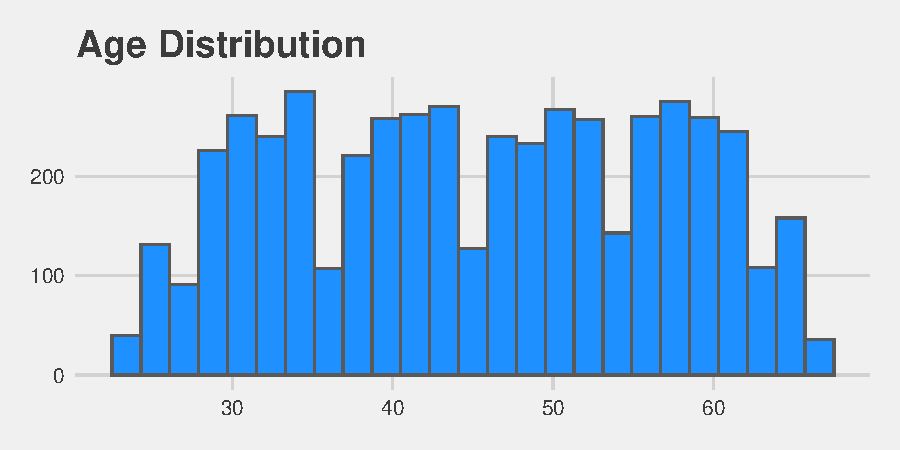
\includegraphics{Bank_Loan_Classification_files/figure-latex/unnamed-chunk-8-1.pdf}

\textbf{Experience Distribution}

\begin{Shaded}
\begin{Highlighting}[]
\CommentTok{# Experience distribution bar plot}
\NormalTok{raw_data }\OperatorTok\StringTok{ }
\StringTok{  }\KeywordTok{ggplot}\NormalTok{(}\KeywordTok{aes}\NormalTok{(}\DataTypeTok{x =}\NormalTok{ experience)) }\OperatorTok{+}
\StringTok{  }\KeywordTok{geom_histogram}\NormalTok{(}\DataTypeTok{stat =} \StringTok{'bin'}\NormalTok{, }\DataTypeTok{binwidth =} \FloatTok{1.8}\NormalTok{, }\DataTypeTok{color =} \StringTok{'#595959'}\NormalTok{, }\DataTypeTok{fill =} \StringTok{'#1E90FF'}\NormalTok{) }\OperatorTok{+}
\StringTok{  }\KeywordTok{labs}\NormalTok{(}\DataTypeTok{title =} \StringTok{"Experience Distribution"}\NormalTok{) }\OperatorTok{+}
\StringTok{  }\KeywordTok{theme_fivethirtyeight}\NormalTok{()}
\end{Highlighting}
\end{Shaded}

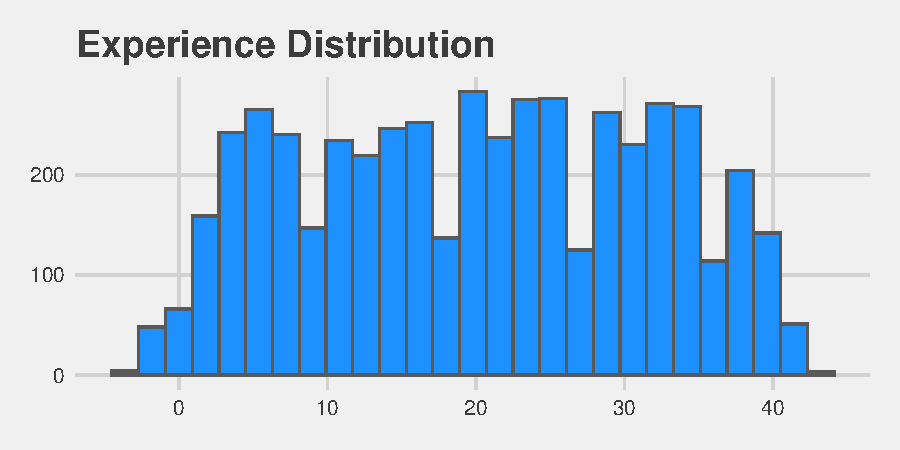
\includegraphics{Bank_Loan_Classification_files/figure-latex/unnamed-chunk-9-1.pdf}

We note that age and experience distributions look similar, They might
be highly correlated. If so, we might have to remove one of the
variables so that our models do not fail.

\textbf{Income Distribution}

\begin{Shaded}
\begin{Highlighting}[]
\CommentTok{# Income Distribution bar plot}
\NormalTok{raw_data }\OperatorTok\StringTok{ }
\StringTok{  }\KeywordTok{ggplot}\NormalTok{(}\KeywordTok{aes}\NormalTok{(}\DataTypeTok{x =}\NormalTok{ income)) }\OperatorTok{+}
\StringTok{  }\KeywordTok{geom_bar}\NormalTok{(}\DataTypeTok{stat =} \StringTok{'bin'}\NormalTok{, }\DataTypeTok{bins =} \DecValTok{40}\NormalTok{, }\DataTypeTok{color =} \StringTok{'#595959'}\NormalTok{, }\DataTypeTok{fill =} \StringTok{'#1E90FF'}\NormalTok{) }\OperatorTok{+}
\StringTok{  }\KeywordTok{labs}\NormalTok{(}\DataTypeTok{title =} \StringTok{"Income Distribution"}\NormalTok{) }\OperatorTok{+}
\StringTok{  }\KeywordTok{theme_fivethirtyeight}\NormalTok{()}
\end{Highlighting}
\end{Shaded}

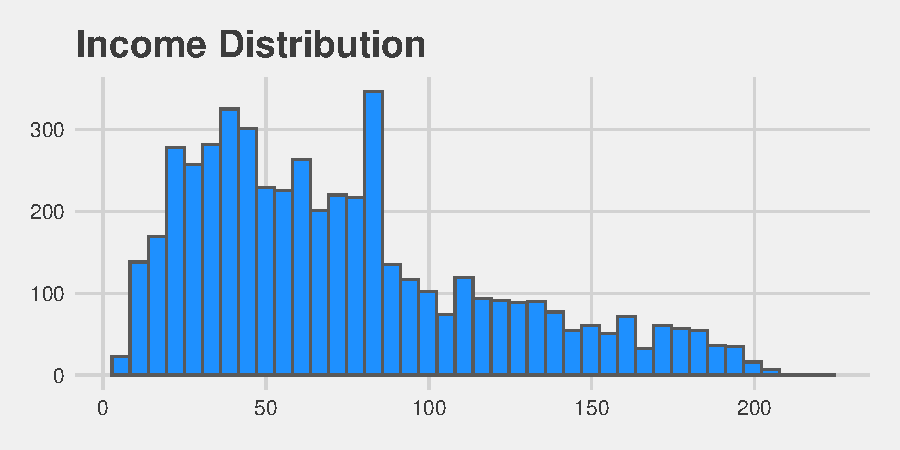
\includegraphics{Bank_Loan_Classification_files/figure-latex/unnamed-chunk-10-1.pdf}

\textbf{Mortgage Distribution}

\begin{Shaded}
\begin{Highlighting}[]
\CommentTok{# Mortgage Distribution bar plot}
\NormalTok{raw_data }\OperatorTok\StringTok{ }
\StringTok{  }\KeywordTok{ggplot}\NormalTok{(}\KeywordTok{aes}\NormalTok{(}\DataTypeTok{x =}\NormalTok{ mortgage)) }\OperatorTok{+}
\StringTok{  }\KeywordTok{geom_bar}\NormalTok{(}\DataTypeTok{stat =} \StringTok{'bin'}\NormalTok{, }\DataTypeTok{color =} \StringTok{'#595959'}\NormalTok{, }\DataTypeTok{fill =} \StringTok{'#1E90FF'}\NormalTok{) }\OperatorTok{+}
\StringTok{  }\KeywordTok{labs}\NormalTok{(}\DataTypeTok{title =} \StringTok{"Mortage Distribution"}\NormalTok{) }\OperatorTok{+}
\StringTok{  }\KeywordTok{theme_fivethirtyeight}\NormalTok{()}
\end{Highlighting}
\end{Shaded}

\begin{verbatim}
## `stat_bin()` using `bins = 30`. Pick better value with `binwidth`.
\end{verbatim}

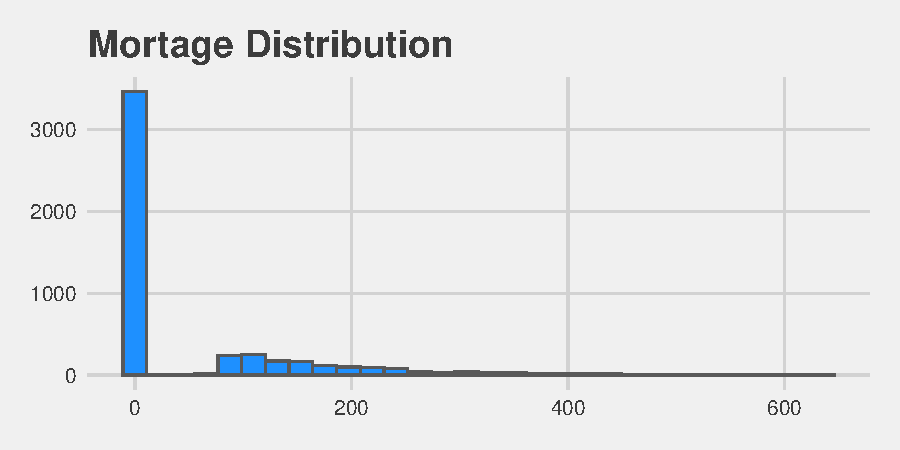
\includegraphics{Bank_Loan_Classification_files/figure-latex/unnamed-chunk-11-1.pdf}

Seems like most people have no mortage (i.e, mortage is 0); So, we
produce another plot removing those without mortgages.

\textbf{Mortgage Distribution exclding people with no mortgages}

\begin{Shaded}
\begin{Highlighting}[]
\CommentTok{# Mortage Distribution bar plot for people with mortgages (exclude 0)}
\NormalTok{raw_data }\OperatorTok\StringTok{ }
\StringTok{  }\KeywordTok{filter}\NormalTok{(mortgage }\OperatorTok{>}\StringTok{ }\DecValTok{0}\NormalTok{) }\OperatorTok
\StringTok{  }\KeywordTok{ggplot}\NormalTok{(}\KeywordTok{aes}\NormalTok{(}\DataTypeTok{x =}\NormalTok{ mortgage)) }\OperatorTok{+}
\StringTok{  }\KeywordTok{geom_bar}\NormalTok{(}\DataTypeTok{stat =} \StringTok{'bin'}\NormalTok{, }\DataTypeTok{bins =} \DecValTok{40}\NormalTok{, }\DataTypeTok{color =} \StringTok{'#595959'}\NormalTok{, }\DataTypeTok{fill =} \StringTok{'#1E90FF'}\NormalTok{) }\OperatorTok{+}
\StringTok{  }\KeywordTok{labs}\NormalTok{(}\DataTypeTok{title =} \StringTok{"Mortgage Distribution"}\NormalTok{) }\OperatorTok{+}
\StringTok{  }\KeywordTok{theme_fivethirtyeight}\NormalTok{()}
\end{Highlighting}
\end{Shaded}

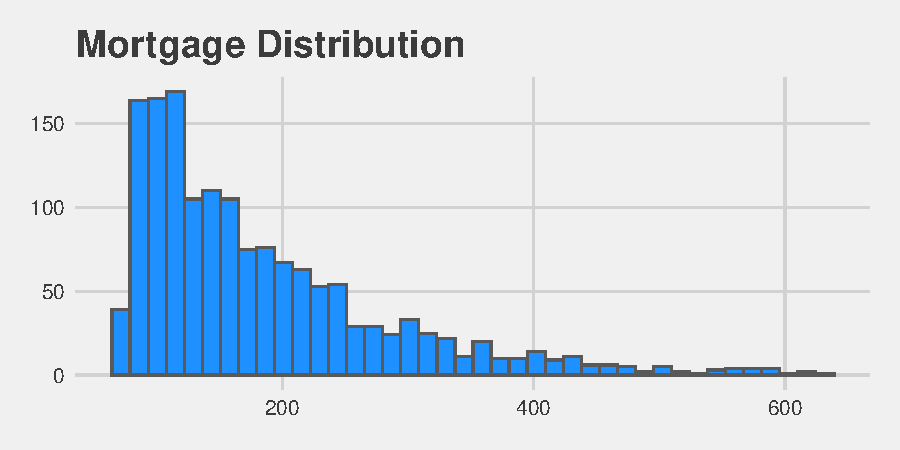
\includegraphics{Bank_Loan_Classification_files/figure-latex/unnamed-chunk-12-1.pdf}

\begin{Shaded}
\begin{Highlighting}[]
\CommentTok{# It is a right skewed distribution}
\end{Highlighting}
\end{Shaded}

\textbf{Credit Card Spending Distribution}

\begin{Shaded}
\begin{Highlighting}[]
\CommentTok{# Credit Card Spending Distribution bar plot for people with mortgages}
\NormalTok{raw_data }\OperatorTok\StringTok{ }
\StringTok{  }\KeywordTok{ggplot}\NormalTok{(}\KeywordTok{aes}\NormalTok{(}\DataTypeTok{x =}\NormalTok{ credit_card_spend)) }\OperatorTok{+}
\StringTok{  }\KeywordTok{geom_bar}\NormalTok{(}\DataTypeTok{stat =} \StringTok{'bin'}\NormalTok{, }\DataTypeTok{bins =} \DecValTok{50}\NormalTok{, }\DataTypeTok{color =} \StringTok{'#595959'}\NormalTok{, }\DataTypeTok{fill =} \StringTok{'#1E90FF'}\NormalTok{) }\OperatorTok{+}
\StringTok{  }\KeywordTok{labs}\NormalTok{(}\DataTypeTok{title =} \StringTok{"Credit Card Spending Distribution"}\NormalTok{) }\OperatorTok{+}
\StringTok{  }\KeywordTok{theme_fivethirtyeight}\NormalTok{()}
\end{Highlighting}
\end{Shaded}

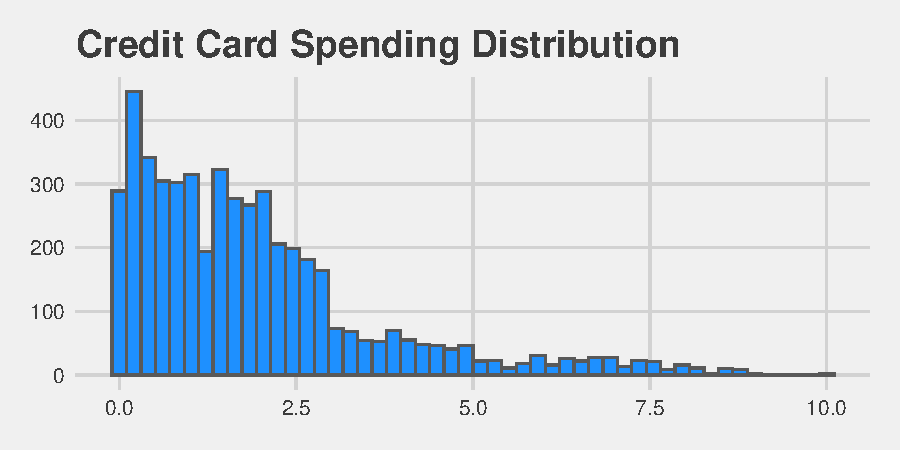
\includegraphics{Bank_Loan_Classification_files/figure-latex/unnamed-chunk-13-1.pdf}

\begin{Shaded}
\begin{Highlighting}[]
\CommentTok{# It is a right skewed distribution}
\end{Highlighting}
\end{Shaded}

\pagebreak

\hypertarget{bivariate-plots}{%
\subsubsection{Bivariate Plots}\label{bivariate-plots}}

\textbf{Personal Loan vs.~CD Account}

\begin{Shaded}
\begin{Highlighting}[]
\CommentTok{# Stacked bar plot to test for Credit Card vs. personal loan}
\NormalTok{raw_data }\OperatorTok\StringTok{ }
\StringTok{  }\KeywordTok{ggplot}\NormalTok{(}\KeywordTok{aes}\NormalTok{(}\DataTypeTok{x =}\NormalTok{ credit_card, }\DataTypeTok{y =}\NormalTok{ personal_loan, }\DataTypeTok{fill =}\NormalTok{ personal_loan)) }\OperatorTok{+}
\StringTok{  }\KeywordTok{geom_bar}\NormalTok{(}\DataTypeTok{stat =} \StringTok{'identity'}\NormalTok{) }\OperatorTok{+}
\StringTok{  }\KeywordTok{coord_flip}\NormalTok{() }\OperatorTok{+}\StringTok{ }
\StringTok{  }\KeywordTok{scale_fill_manual}\NormalTok{(}\DataTypeTok{values=}\KeywordTok{c}\NormalTok{(}\StringTok{'#DE3533'}\NormalTok{,}\StringTok{'#51A8C9'}\NormalTok{)) }\OperatorTok{+}
\StringTok{  }\KeywordTok{labs}\NormalTok{(}\DataTypeTok{title =} \StringTok{"Personal Loan vs. CD Account"}\NormalTok{) }\OperatorTok{+}
\StringTok{  }\KeywordTok{theme_fivethirtyeight}\NormalTok{() }\OperatorTok{+}\StringTok{ }
\StringTok{  }\KeywordTok{theme}\NormalTok{(}\DataTypeTok{axis.title =} \KeywordTok{element_text}\NormalTok{()) }\OperatorTok{+}
\StringTok{  }\KeywordTok{xlab}\NormalTok{(}\StringTok{'Credit Card'}\NormalTok{)}
\end{Highlighting}
\end{Shaded}

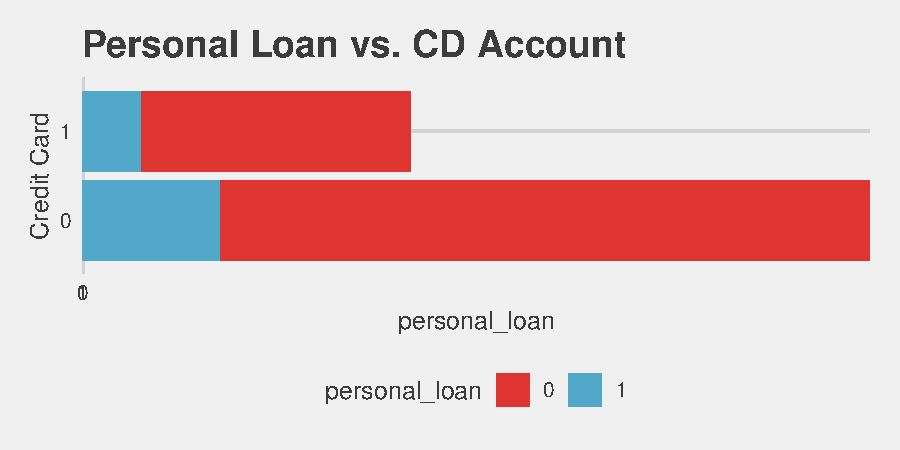
\includegraphics{Bank_Loan_Classification_files/figure-latex/unnamed-chunk-14-1.pdf}

We can observe that people who do not have a credit card are more likey
to get personal loan.

\textbf{Personal Loan vs.~Credit Card Spending}

\begin{Shaded}
\begin{Highlighting}[]
\CommentTok{# Bar plot to test for Credit Card Spending vs. personal loan}
\NormalTok{raw_data }\OperatorTok\StringTok{ }
\StringTok{  }\KeywordTok{ggplot}\NormalTok{(}\KeywordTok{aes}\NormalTok{(}\DataTypeTok{x =}\NormalTok{ credit_card_spend, }\DataTypeTok{y =}\NormalTok{ personal_loan, }\DataTypeTok{fill =}\NormalTok{ personal_loan)) }\OperatorTok{+}
\StringTok{  }\KeywordTok{geom_bar}\NormalTok{(}\DataTypeTok{stat =} \StringTok{'identity'}\NormalTok{) }\OperatorTok{+}
\StringTok{  }\KeywordTok{coord_flip}\NormalTok{() }\OperatorTok{+}\StringTok{ }
\StringTok{  }\KeywordTok{scale_fill_manual}\NormalTok{(}\DataTypeTok{values=}\KeywordTok{c}\NormalTok{(}\StringTok{'#DE3533'}\NormalTok{,}\StringTok{'#51A8C9'}\NormalTok{)) }\OperatorTok{+}
\StringTok{  }\KeywordTok{labs}\NormalTok{(}\DataTypeTok{title =} \StringTok{"Personal Loan vs. Credit Card Spending"}\NormalTok{) }\OperatorTok{+}
\StringTok{  }\KeywordTok{theme_fivethirtyeight}\NormalTok{() }\OperatorTok{+}
\StringTok{  }\KeywordTok{theme}\NormalTok{(}\DataTypeTok{axis.title =} \KeywordTok{element_text}\NormalTok{()) }\OperatorTok{+}
\StringTok{  }\KeywordTok{xlab}\NormalTok{(}\StringTok{'Credit Card Spending'}\NormalTok{)}
\end{Highlighting}
\end{Shaded}

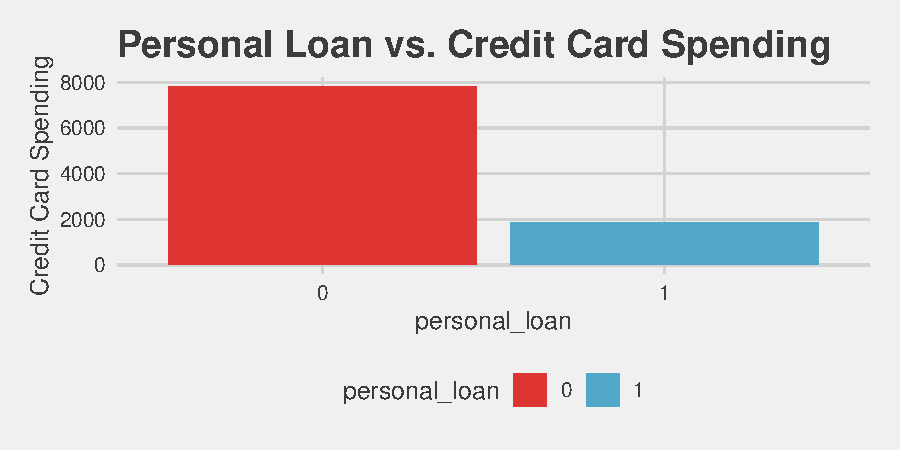
\includegraphics{Bank_Loan_Classification_files/figure-latex/unnamed-chunk-15-1.pdf}

We can observe that people whose credit card spending is high do not
generally borrow loans

\textbf{Personal Loan vs.~Income}

\begin{Shaded}
\begin{Highlighting}[]
\CommentTok{# Bar plot to test for Income vs. personal loan}
\NormalTok{raw_data }\OperatorTok\StringTok{ }
\StringTok{  }\KeywordTok{ggplot}\NormalTok{(}\KeywordTok{aes}\NormalTok{(}\DataTypeTok{x =}\NormalTok{ income, }\DataTypeTok{y =}\NormalTok{ personal_loan, }\DataTypeTok{fill =}\NormalTok{ personal_loan)) }\OperatorTok{+}
\StringTok{  }\KeywordTok{geom_bar}\NormalTok{(}\DataTypeTok{stat =} \StringTok{'identity'}\NormalTok{) }\OperatorTok{+}
\StringTok{  }\KeywordTok{coord_flip}\NormalTok{() }\OperatorTok{+}\StringTok{ }
\StringTok{  }\KeywordTok{scale_fill_manual}\NormalTok{(}\DataTypeTok{values=}\KeywordTok{c}\NormalTok{(}\StringTok{'#DE3533'}\NormalTok{,}\StringTok{'#51A8C9'}\NormalTok{)) }\OperatorTok{+}
\StringTok{  }\KeywordTok{labs}\NormalTok{(}\DataTypeTok{title =} \StringTok{"Personal Loan vs. Income"}\NormalTok{) }\OperatorTok{+}
\StringTok{  }\KeywordTok{theme_fivethirtyeight}\NormalTok{() }\OperatorTok{+}
\StringTok{  }\KeywordTok{theme}\NormalTok{(}\DataTypeTok{axis.title =} \KeywordTok{element_text}\NormalTok{()) }\OperatorTok{+}
\StringTok{  }\KeywordTok{xlab}\NormalTok{(}\StringTok{'Income'}\NormalTok{)}
\end{Highlighting}
\end{Shaded}

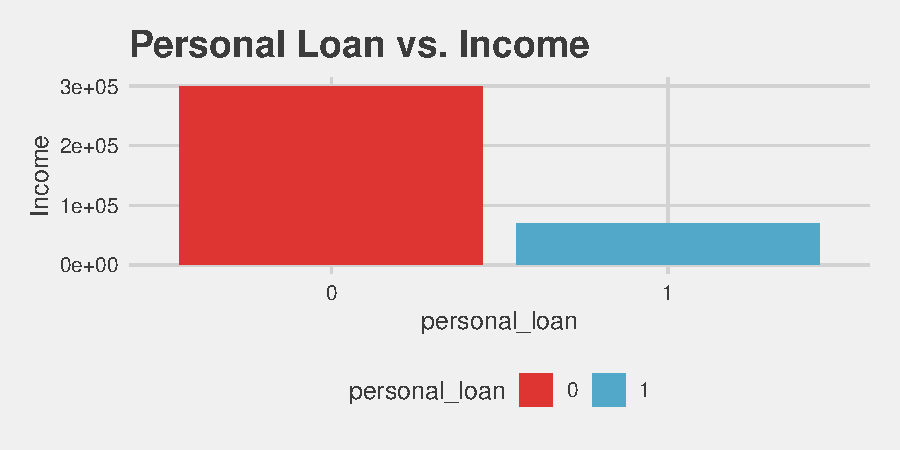
\includegraphics{Bank_Loan_Classification_files/figure-latex/unnamed-chunk-16-1.pdf}

We can observe that people with higher incomes do not generally borrow
loans

\textbf{Personal Loan vs.~Family}

\begin{Shaded}
\begin{Highlighting}[]
\CommentTok{# Stacked bar plot to test for family vs. personal loan}
\NormalTok{raw_data }\OperatorTok\StringTok{ }
\StringTok{  }\KeywordTok{ggplot}\NormalTok{(}\KeywordTok{aes}\NormalTok{(}\DataTypeTok{x =}\NormalTok{ family, }\DataTypeTok{y =}\NormalTok{ personal_loan, }\DataTypeTok{fill =}\NormalTok{ personal_loan)) }\OperatorTok{+}
\StringTok{  }\KeywordTok{geom_bar}\NormalTok{(}\DataTypeTok{stat =} \StringTok{'identity'}\NormalTok{) }\OperatorTok{+}
\StringTok{  }\KeywordTok{coord_flip}\NormalTok{() }\OperatorTok{+}\StringTok{ }
\StringTok{  }\KeywordTok{scale_fill_manual}\NormalTok{(}\DataTypeTok{values=}\KeywordTok{c}\NormalTok{(}\StringTok{'#DE3533'}\NormalTok{,}\StringTok{'#51A8C9'}\NormalTok{)) }\OperatorTok{+}
\StringTok{  }\KeywordTok{labs}\NormalTok{(}\DataTypeTok{title =} \StringTok{"Personal Loan vs. Family"}\NormalTok{) }\OperatorTok{+}
\StringTok{  }\KeywordTok{theme_fivethirtyeight}\NormalTok{() }\OperatorTok{+}
\StringTok{  }\KeywordTok{theme}\NormalTok{(}\DataTypeTok{axis.title =} \KeywordTok{element_text}\NormalTok{()) }\OperatorTok{+}
\StringTok{  }\KeywordTok{xlab}\NormalTok{(}\StringTok{'Family Members'}\NormalTok{)}
\end{Highlighting}
\end{Shaded}

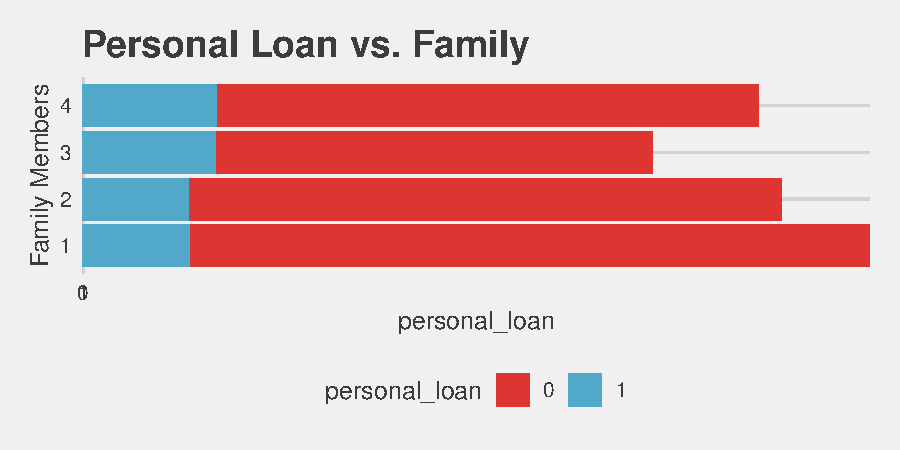
\includegraphics{Bank_Loan_Classification_files/figure-latex/unnamed-chunk-17-1.pdf}

We observe the differnce in whether or not people take loans based on
the number of family members.

\textbf{Personal Loan vs.~Education}

\begin{Shaded}
\begin{Highlighting}[]
\CommentTok{# Stacked bar plot to test for education vs. personal loan}
\NormalTok{raw_data }\OperatorTok\StringTok{ }
\StringTok{  }\KeywordTok{ggplot}\NormalTok{(}\KeywordTok{aes}\NormalTok{(}\DataTypeTok{x =}\NormalTok{ education, }\DataTypeTok{y =}\NormalTok{ personal_loan, }\DataTypeTok{fill =}\NormalTok{ personal_loan)) }\OperatorTok{+}
\StringTok{  }\KeywordTok{geom_bar}\NormalTok{(}\DataTypeTok{stat =} \StringTok{'identity'}\NormalTok{) }\OperatorTok{+}
\StringTok{  }\KeywordTok{coord_flip}\NormalTok{() }\OperatorTok{+}\StringTok{ }
\StringTok{  }\KeywordTok{scale_fill_manual}\NormalTok{(}\DataTypeTok{values=}\KeywordTok{c}\NormalTok{(}\StringTok{'#DE3533'}\NormalTok{,}\StringTok{'#51A8C9'}\NormalTok{)) }\OperatorTok{+}
\StringTok{  }\KeywordTok{labs}\NormalTok{(}\DataTypeTok{title =} \StringTok{"Personal Loan vs. Education"}\NormalTok{) }\OperatorTok{+}
\StringTok{  }\KeywordTok{theme_fivethirtyeight}\NormalTok{() }\OperatorTok{+}
\StringTok{  }\KeywordTok{theme}\NormalTok{(}\DataTypeTok{axis.title =} \KeywordTok{element_text}\NormalTok{()) }\OperatorTok{+}
\StringTok{  }\KeywordTok{xlab}\NormalTok{(}\StringTok{'Education Level'}\NormalTok{)}
\end{Highlighting}
\end{Shaded}

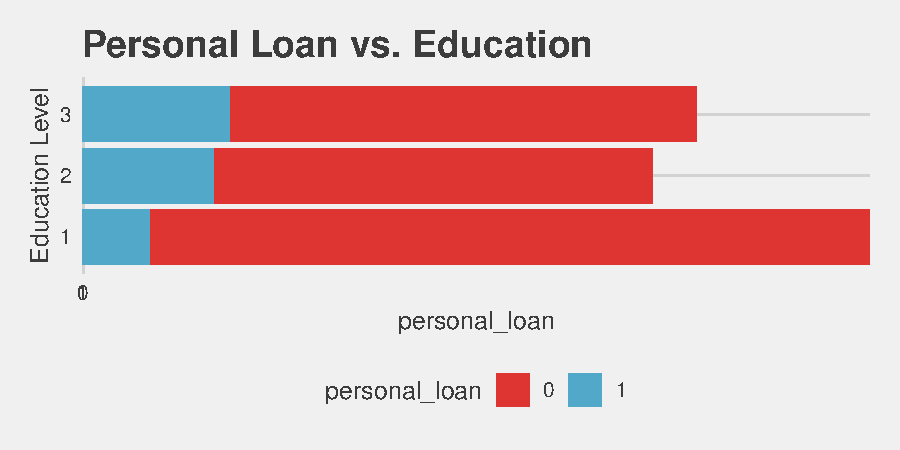
\includegraphics{Bank_Loan_Classification_files/figure-latex/unnamed-chunk-18-1.pdf}

We can observe some differneces.

\textbf{Personal Loan vs.~Online}

\begin{Shaded}
\begin{Highlighting}[]
\CommentTok{# Stacked bar plot to test for online vs. personal loan}
\NormalTok{raw_data }\OperatorTok\StringTok{ }
\StringTok{  }\KeywordTok{ggplot}\NormalTok{(}\KeywordTok{aes}\NormalTok{(}\DataTypeTok{x =}\NormalTok{ online, }\DataTypeTok{y =}\NormalTok{ personal_loan, }\DataTypeTok{fill =}\NormalTok{ personal_loan)) }\OperatorTok{+}
\StringTok{  }\KeywordTok{geom_bar}\NormalTok{(}\DataTypeTok{stat =} \StringTok{'identity'}\NormalTok{) }\OperatorTok{+}
\StringTok{  }\KeywordTok{coord_flip}\NormalTok{() }\OperatorTok{+}\StringTok{ }
\StringTok{  }\KeywordTok{scale_fill_manual}\NormalTok{(}\DataTypeTok{values=}\KeywordTok{c}\NormalTok{(}\StringTok{'#DE3533'}\NormalTok{,}\StringTok{'#51A8C9'}\NormalTok{)) }\OperatorTok{+}
\StringTok{  }\KeywordTok{labs}\NormalTok{(}\DataTypeTok{title =} \StringTok{"Personal Loan vs. Online"}\NormalTok{) }\OperatorTok{+}
\StringTok{  }\KeywordTok{theme_fivethirtyeight}\NormalTok{() }\OperatorTok{+}
\StringTok{  }\KeywordTok{theme}\NormalTok{(}\DataTypeTok{axis.title =} \KeywordTok{element_text}\NormalTok{()) }\OperatorTok{+}
\StringTok{  }\KeywordTok{xlab}\NormalTok{(}\StringTok{'Online'}\NormalTok{)}
\end{Highlighting}
\end{Shaded}

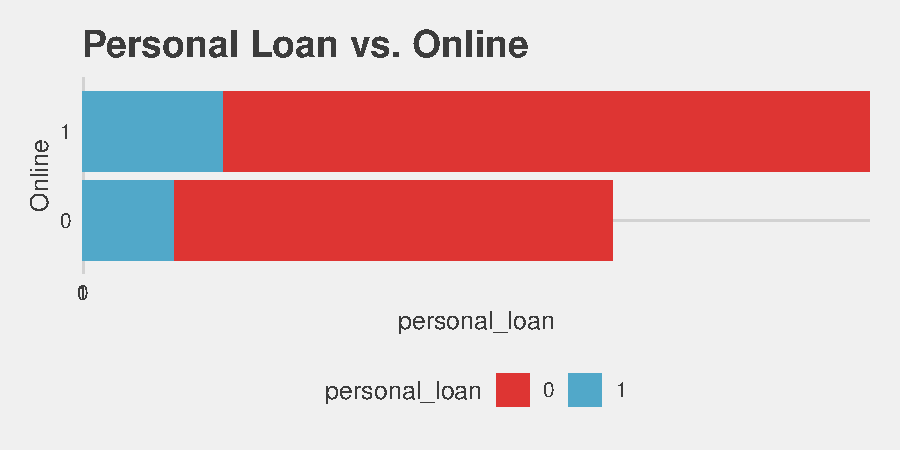
\includegraphics{Bank_Loan_Classification_files/figure-latex/unnamed-chunk-19-1.pdf}

We can observe the differnce in whether or not people borrow loans based
on whether they engage in online banking.

\textbf{Personal Loan vs.~Securities Account}

\begin{Shaded}
\begin{Highlighting}[]
\CommentTok{# Stacked bar plot to test for Securites Account vs. personal loan}
\NormalTok{raw_data }\OperatorTok\StringTok{ }
\StringTok{  }\KeywordTok{ggplot}\NormalTok{(}\KeywordTok{aes}\NormalTok{(}\DataTypeTok{x =}\NormalTok{ securities_account, }\DataTypeTok{y =}\NormalTok{ personal_loan, }\DataTypeTok{fill =}\NormalTok{ personal_loan)) }\OperatorTok{+}
\StringTok{  }\KeywordTok{geom_bar}\NormalTok{(}\DataTypeTok{stat =} \StringTok{'identity'}\NormalTok{) }\OperatorTok{+}
\StringTok{  }\KeywordTok{coord_flip}\NormalTok{() }\OperatorTok{+}\StringTok{ }
\StringTok{  }\KeywordTok{scale_fill_manual}\NormalTok{(}\DataTypeTok{values=}\KeywordTok{c}\NormalTok{(}\StringTok{'#DE3533'}\NormalTok{,}\StringTok{'#51A8C9'}\NormalTok{)) }\OperatorTok{+}
\StringTok{  }\KeywordTok{labs}\NormalTok{(}\DataTypeTok{title =} \StringTok{"Personal Loan vs. Securities Account"}\NormalTok{) }\OperatorTok{+}
\StringTok{  }\KeywordTok{theme_fivethirtyeight}\NormalTok{() }\OperatorTok{+}
\StringTok{  }\KeywordTok{theme}\NormalTok{(}\DataTypeTok{axis.title =} \KeywordTok{element_text}\NormalTok{()) }\OperatorTok{+}
\StringTok{  }\KeywordTok{xlab}\NormalTok{(}\StringTok{'Securities Account'}\NormalTok{)}
\end{Highlighting}
\end{Shaded}

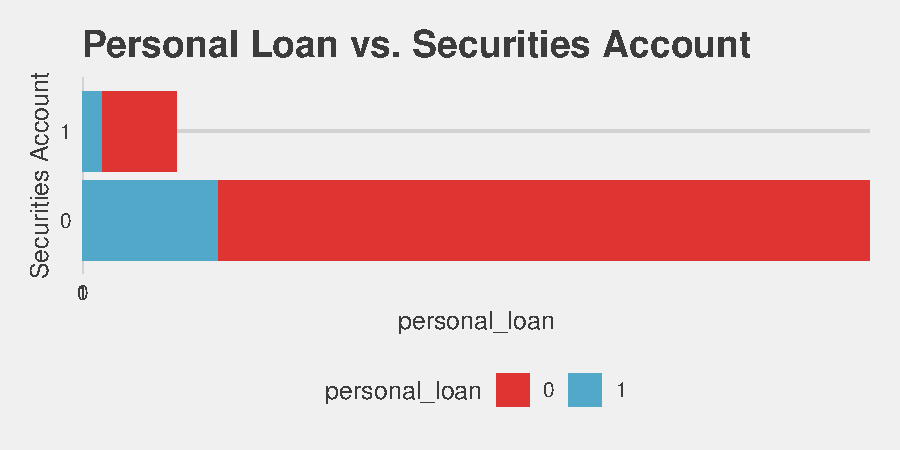
\includegraphics{Bank_Loan_Classification_files/figure-latex/unnamed-chunk-20-1.pdf}

We can observe that people are more likely to a loan if they do not have
a securities account

\textbf{Personal Loan vs.~CD Account}

\begin{Shaded}
\begin{Highlighting}[]
\CommentTok{# Stacked bar plot to test for CD Account vs. personal loan}
\NormalTok{raw_data }\OperatorTok\StringTok{ }
\StringTok{  }\KeywordTok{ggplot}\NormalTok{(}\KeywordTok{aes}\NormalTok{(}\DataTypeTok{x =}\NormalTok{ cd_account, }\DataTypeTok{y =}\NormalTok{ personal_loan, }\DataTypeTok{fill =}\NormalTok{ personal_loan)) }\OperatorTok{+}
\StringTok{  }\KeywordTok{geom_bar}\NormalTok{(}\DataTypeTok{stat =} \StringTok{'identity'}\NormalTok{) }\OperatorTok{+}
\StringTok{  }\KeywordTok{coord_flip}\NormalTok{() }\OperatorTok{+}\StringTok{ }
\StringTok{  }\KeywordTok{scale_fill_manual}\NormalTok{(}\DataTypeTok{values=}\KeywordTok{c}\NormalTok{(}\StringTok{'#DE3533'}\NormalTok{,}\StringTok{'#51A8C9'}\NormalTok{)) }\OperatorTok{+}
\StringTok{  }\KeywordTok{labs}\NormalTok{(}\DataTypeTok{title =} \StringTok{"Personal Loan vs. CD Account"}\NormalTok{) }\OperatorTok{+}
\StringTok{  }\KeywordTok{theme_fivethirtyeight}\NormalTok{() }\OperatorTok{+}
\StringTok{  }\KeywordTok{theme}\NormalTok{(}\DataTypeTok{axis.title =} \KeywordTok{element_text}\NormalTok{()) }\OperatorTok{+}
\StringTok{  }\KeywordTok{xlab}\NormalTok{(}\StringTok{'CD Account'}\NormalTok{)}
\end{Highlighting}
\end{Shaded}

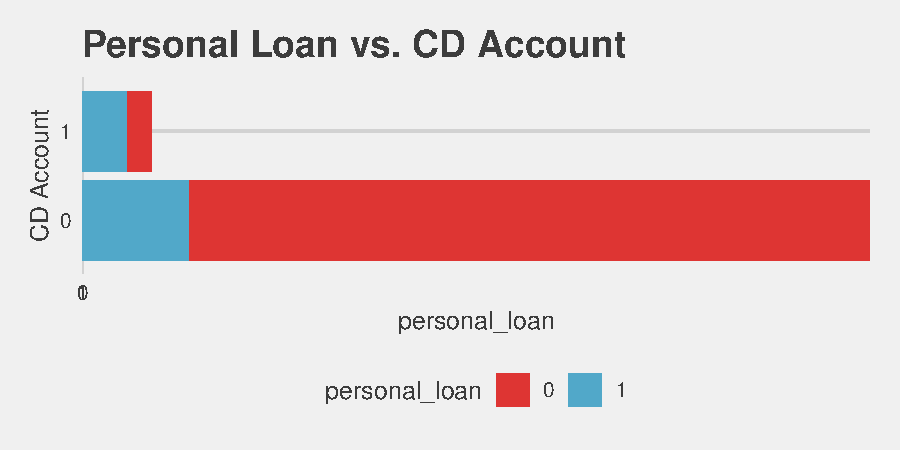
\includegraphics{Bank_Loan_Classification_files/figure-latex/unnamed-chunk-21-1.pdf}
We can observe that people are more likely to a loan if they do not have
a securities account

\pagebreak

\hypertarget{correlation-heatmap}{%
\subsubsection{Correlation Heatmap}\label{correlation-heatmap}}

We generate a heatmap of \textbf{correlations} among the numeric
variables in the dataset.

\begin{Shaded}
\begin{Highlighting}[]
\CommentTok{# Correlation plot for the numeric columns}
\NormalTok{numeric_vaiables <-}\StringTok{ }\KeywordTok{c}\NormalTok{(}\StringTok{'age'}\NormalTok{, }\StringTok{'experience'}\NormalTok{, }\StringTok{'income'}\NormalTok{, }\StringTok{'mortgage'}\NormalTok{, }\StringTok{'credit_card_spend'}\NormalTok{)}

\CommentTok{# Using ggcor from GGally package to produce correlation heatmap}
\KeywordTok{ggcorr}\NormalTok{(raw_data[, numeric_vaiables], }\DataTypeTok{nbreaks =} \DecValTok{7}\NormalTok{, }
       \DataTypeTok{low =} \StringTok{"#1E90FF"}\NormalTok{, }\DataTypeTok{mid =} \StringTok{"#AAAAAA"}\NormalTok{, }\DataTypeTok{high =} \StringTok{"#F21A00"}\NormalTok{,}
       \DataTypeTok{label =} \OtherTok{TRUE}\NormalTok{, }\DataTypeTok{label_size =} \DecValTok{7}\NormalTok{, }\DataTypeTok{label_color=}\StringTok{'black'}\NormalTok{,}
       \DataTypeTok{legend.position =} \StringTok{'left'}\NormalTok{) }\OperatorTok{+}
\StringTok{  }\KeywordTok{theme_gray}\NormalTok{()}
\end{Highlighting}
\end{Shaded}

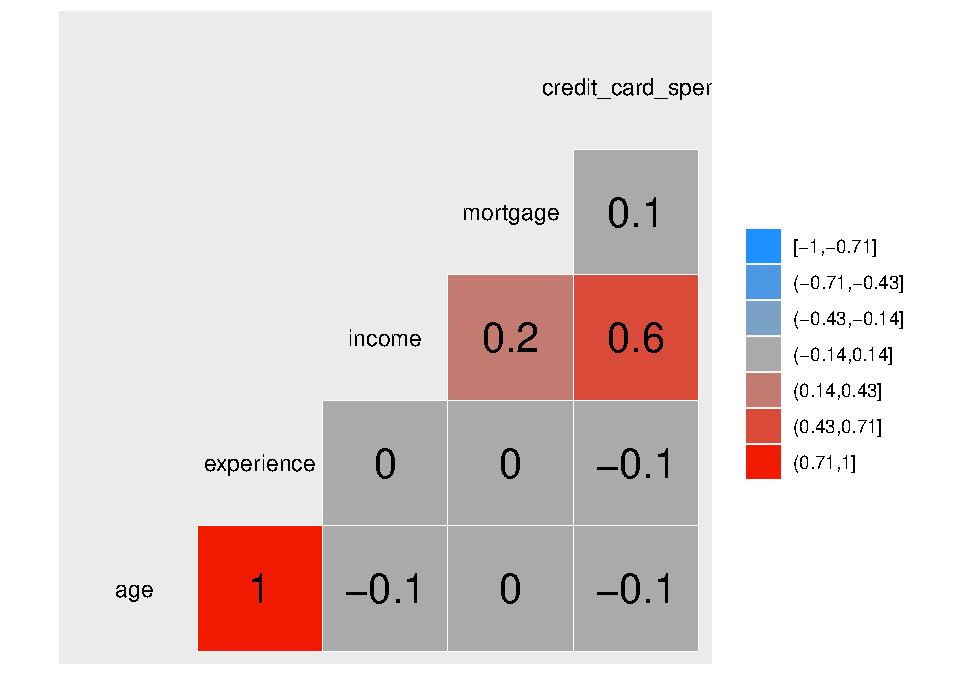
\includegraphics{Bank_Loan_Classification_files/figure-latex/unnamed-chunk-22-1.pdf}

We can observe that age and experience are \textbf{highly correlated},
Hence, we have to remove experience.

\pagebreak

\hypertarget{data-preprocessing}{%
\section{Data Preprocessing}\label{data-preprocessing}}

\textbf{Remove the experience variable}

\begin{Shaded}
\begin{Highlighting}[]
\CommentTok{# Removing Experience variable as it is highly correlated with age and will mess with our models if left}
\NormalTok{raw_data}\OperatorTok{$}\NormalTok{experience <-}\StringTok{ }\OtherTok{NULL}

\CommentTok{# Data Splitting - Training Data = 60%, Validation Data = 20% & Testing Data = 20%}
\end{Highlighting}
\end{Shaded}

\hypertarget{split-the-data}{%
\subsection{Split the data}\label{split-the-data}}

\textbf{Splitting the dataset into train, validation and test} We split
the dataset into three sets:

\begin{verbatim}
1. Training    60%  | To train the models on
2. Validation  20%  | To tune and test our models to select best models
3. Testing     20%  | To evaluate the final model
\end{verbatim}

\begin{Shaded}
\begin{Highlighting}[]
\CommentTok{# Setting seed for reproducibility of results}
\CommentTok{# Remove sample.kind = "Rounding" if R version < 3.5}
\KeywordTok{set.seed}\NormalTok{(}\DecValTok{7}\NormalTok{, }\DataTypeTok{sample.kind =} \StringTok{"Rounding"}\NormalTok{)}
\end{Highlighting}
\end{Shaded}

\begin{verbatim}
## Warning in set.seed(7, sample.kind = "Rounding"): non-uniform 'Rounding' sampler
## used
\end{verbatim}

\begin{Shaded}
\begin{Highlighting}[]
\CommentTok{# sample into three sets to create indices for train, validation, test sets}
\NormalTok{idx <-}\StringTok{ }\KeywordTok{sample}\NormalTok{(}\KeywordTok{seq}\NormalTok{(}\DecValTok{1}\NormalTok{, }\DecValTok{3}\NormalTok{), }\DataTypeTok{size =} \KeywordTok{nrow}\NormalTok{(raw_data), }\DataTypeTok{replace =} \OtherTok{TRUE}\NormalTok{, }\DataTypeTok{prob =} \KeywordTok{c}\NormalTok{(.}\DecValTok{6}\NormalTok{, }\FloatTok{.2}\NormalTok{, }\FloatTok{.2}\NormalTok{))}

\CommentTok{# Split the data into three sets}
\NormalTok{raw_train <-}\StringTok{ }\NormalTok{raw_data[idx }\OperatorTok{==}\StringTok{ }\DecValTok{1}\NormalTok{,]}
\NormalTok{raw_val <-}\StringTok{ }\NormalTok{raw_data[idx }\OperatorTok{==}\StringTok{ }\DecValTok{2}\NormalTok{,]}
\NormalTok{raw_test <-}\StringTok{ }\NormalTok{raw_data[idx }\OperatorTok{==}\StringTok{ }\DecValTok{3}\NormalTok{,]}
\end{Highlighting}
\end{Shaded}

\textbf{Standardizing the data}

We have seen that the numeric data \textbf{ranges} are very different.
So to bring them into a similar range, we standardize the data. i.e., we
scale and centre the dataset.

\begin{Shaded}
\begin{Highlighting}[]
\CommentTok{# Standardizing the numeric varaibles as we've seen that the ranges of numerical variables vary quite a bit}
\CommentTok{# Using preProcess from caret package}
\NormalTok{(norm.values <-}\StringTok{ }\KeywordTok{preProcess}\NormalTok{(raw_train, }\DataTypeTok{method=}\KeywordTok{c}\NormalTok{(}\StringTok{"center"}\NormalTok{, }\StringTok{"scale"}\NormalTok{)))}
\end{Highlighting}
\end{Shaded}

\begin{verbatim}
## Created from 3012 samples and 11 variables
## 
## Pre-processing:
##   - centered (4)
##   - ignored (7)
##   - scaled (4)
\end{verbatim}

\begin{Shaded}
\begin{Highlighting}[]
\CommentTok{# Apply the preProcess params to the dat using preProcess.predict}
\NormalTok{train <-}\StringTok{ }\KeywordTok{predict}\NormalTok{(norm.values, raw_train)}
\NormalTok{val <-}\StringTok{ }\KeywordTok{predict}\NormalTok{(norm.values, raw_val)}
\NormalTok{test <-}\StringTok{ }\KeywordTok{predict}\NormalTok{(norm.values, raw_test)}
\end{Highlighting}
\end{Shaded}

\pagebreak

\textbf{Summary of normalized data}

\begin{Shaded}
\begin{Highlighting}[]
\CommentTok{# Check the new ranges}
\KeywordTok{summary}\NormalTok{(train)}
\end{Highlighting}
\end{Shaded}

\begin{verbatim}
##       age               income        family  credit_card_spend education
##  Min.   :-1.96297   Min.   :-1.4310   1:877   Min.   :-1.1181   1:1295   
##  1st Qu.:-0.91063   1st Qu.:-0.7584   2:750   1st Qu.:-0.7149   2: 828   
##  Median :-0.03369   Median :-0.2160   3:628   Median :-0.1965   3: 889   
##  Mean   : 0.00000   Mean   : 0.0000   4:757   Mean   : 0.0000            
##  3rd Qu.: 0.84326   3rd Qu.: 0.5217           3rd Qu.: 0.3363            
##  Max.   : 1.89559   Max.   : 3.1254           Max.   : 4.2387            
##     mortgage       personal_loan securities_account cd_account online  
##  Min.   :-0.5555   0:2724        0:2704             0:2834     0:1205  
##  1st Qu.:-0.5555   1: 288        1: 308             1: 178     1:1807  
##  Median :-0.5555                                                       
##  Mean   : 0.0000                                                       
##  3rd Qu.: 0.4367                                                       
##  Max.   : 5.5668                                                       
##  credit_card
##  0:2157     
##  1: 855     
##             
##             
##             
## 
\end{verbatim}

\pagebreak

\hypertarget{model-building}{%
\section{Model Building}\label{model-building}}

First, we define a function to produce neat confusion matrix plots using
\textbf{ggcorr from GGally} library. This library is built on top of the
ggplot2 library.

\begin{Shaded}
\begin{Highlighting}[]
\CommentTok{# Helper function to draw the confusion matrix using ggplot}
\NormalTok{prettyConfusion <-}\StringTok{ }\ControlFlowTok{function}\NormalTok{(results)\{}
  \CommentTok{# Convert the results from confusionMatrix toa  data frame}
\NormalTok{  table <-}\StringTok{ }\KeywordTok{data.frame}\NormalTok{(results}\OperatorTok{$}\NormalTok{table)}
  
  \CommentTok{# Calcualte Proportions and Predicted columns}
\NormalTok{  plotTable <-}\StringTok{ }\NormalTok{table }\OperatorTok
\StringTok{    }\KeywordTok{mutate}\NormalTok{(}\DataTypeTok{Predicted =} \KeywordTok{ifelse}\NormalTok{(table}\OperatorTok{$}\NormalTok{Prediction }\OperatorTok{==}\StringTok{ }\NormalTok{table}\OperatorTok{$}\NormalTok{Reference, }\StringTok{"Correct"}\NormalTok{, }\StringTok{"Wrong"}\NormalTok{)) }\OperatorTok
\StringTok{    }\KeywordTok{group_by}\NormalTok{(Reference) }\OperatorTok
\StringTok{    }\KeywordTok{mutate}\NormalTok{(}\DataTypeTok{Proportion =}\NormalTok{ Freq}\OperatorTok{/}\KeywordTok{sum}\NormalTok{(Freq))}
  
  \CommentTok{# Fill alpha relative to sensitivity/specificity by }
  \CommentTok{# proportional outcomes within reference groups}
  \KeywordTok{ggplot}\NormalTok{(plotTable, }\KeywordTok{aes}\NormalTok{(Reference, Prediction, }\DataTypeTok{fill =}\NormalTok{ Predicted, }\DataTypeTok{alpha =}\NormalTok{ Proportion)) }\OperatorTok{+}
\StringTok{    }\KeywordTok{geom_tile}\NormalTok{() }\OperatorTok{+}
\StringTok{    }\KeywordTok{geom_text}\NormalTok{(}\KeywordTok{aes}\NormalTok{(}\DataTypeTok{label =}\NormalTok{ Freq), }\DataTypeTok{vjust =} \FloatTok{.5}\NormalTok{, }\DataTypeTok{fontface  =} \StringTok{"bold"}\NormalTok{, }\DataTypeTok{size=}\DecValTok{10}\NormalTok{) }\OperatorTok{+}
\StringTok{    }\KeywordTok{scale_fill_manual}\NormalTok{(}\DataTypeTok{values =} \KeywordTok{c}\NormalTok{(}\DataTypeTok{Correct =} \StringTok{"springgreen2"}\NormalTok{, }\DataTypeTok{Wrong =} \StringTok{"orangered2"}\NormalTok{)) }\OperatorTok{+}
\StringTok{    }\KeywordTok{theme_bw}\NormalTok{() }\OperatorTok{+}
\StringTok{    }\KeywordTok{xlim}\NormalTok{(}\KeywordTok{rev}\NormalTok{(}\KeywordTok{levels}\NormalTok{(table}\OperatorTok{$}\NormalTok{Reference))) }\OperatorTok{+}
\StringTok{    }\KeywordTok{theme_map}\NormalTok{() }\OperatorTok{+}
\StringTok{    }\KeywordTok{theme}\NormalTok{(}\DataTypeTok{legend.position =} \StringTok{"none"}\NormalTok{)}
\NormalTok{\}}
\end{Highlighting}
\end{Shaded}

\textbf{Logistic Regression Classifier}

\begin{Shaded}
\begin{Highlighting}[]
\CommentTok{##--------Logistic Regression Classifier----------##}
\CommentTok{# train}
\NormalTok{lr <-}\StringTok{ }\KeywordTok{train}\NormalTok{(personal_loan }\OperatorTok{~}\StringTok{ }\NormalTok{., }\DataTypeTok{data =}\NormalTok{ train, }\DataTypeTok{method =} \StringTok{"glm"}\NormalTok{, }\DataTypeTok{family =}\NormalTok{ binomial)}

\CommentTok{# predictions}
\NormalTok{pred_lr <-}\StringTok{ }\KeywordTok{predict}\NormalTok{(lr, val)}

\CommentTok{# Accuracy of the model}
\NormalTok{(acc_lr <-}\StringTok{ }\KeywordTok{mean}\NormalTok{(pred_lr }\OperatorTok{==}\StringTok{ }\NormalTok{val}\OperatorTok{$}\NormalTok{personal_loan))}
\end{Highlighting}
\end{Shaded}

\begin{verbatim}
## [1] 0.9602851
\end{verbatim}

\begin{Shaded}
\begin{Highlighting}[]
\CommentTok{# Generate Confusion Matrix of the model}
\NormalTok{results_lr <-}\StringTok{ }\KeywordTok{confusionMatrix}\NormalTok{(pred_lr, val}\OperatorTok{$}\NormalTok{personal_loan, }\DataTypeTok{positive=}\StringTok{"1"}\NormalTok{)}

\CommentTok{# F1 Score}
\NormalTok{(f1_lr <-}\StringTok{ }\NormalTok{results_lr}\OperatorTok{$}\NormalTok{byClass[}\StringTok{'F1'}\NormalTok{])}
\end{Highlighting}
\end{Shaded}

\begin{verbatim}
##        F1 
## 0.7719298
\end{verbatim}

\begin{Shaded}
\begin{Highlighting}[]
\CommentTok{# Draw a pretty confusion matrix using the custom helper function}
\KeywordTok{prettyConfusion}\NormalTok{(results_lr)}
\end{Highlighting}
\end{Shaded}

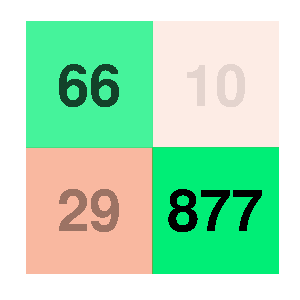
\includegraphics{Bank_Loan_Classification_files/figure-latex/unnamed-chunk-28-1.pdf}

Accuracy: 96.0285132\\
F1-Score: 0.7719298

\textbf{Naīve Bayes Classifier}

\begin{Shaded}
\begin{Highlighting}[]
\CommentTok{##------------Naive Bayes Classifier--------------##}
\CommentTok{# train}
\NormalTok{nb <-}\StringTok{ }\KeywordTok{train}\NormalTok{(personal_loan }\OperatorTok{~}\StringTok{ }\NormalTok{., }\DataTypeTok{data =}\NormalTok{ train, }\DataTypeTok{method =} \StringTok{"nb"}\NormalTok{)}

\CommentTok{# predictions}
\NormalTok{pred_nb <-}\StringTok{ }\KeywordTok{predict}\NormalTok{(nb, val)}

\CommentTok{# Accuracy of the model}
\NormalTok{(acc_nb <-}\StringTok{ }\KeywordTok{mean}\NormalTok{(pred_nb }\OperatorTok{==}\StringTok{ }\NormalTok{val}\OperatorTok{$}\NormalTok{personal_loan))}
\end{Highlighting}
\end{Shaded}

\begin{verbatim}
## [1] 0.907332
\end{verbatim}

\begin{Shaded}
\begin{Highlighting}[]
\CommentTok{# Generate Confusion Matrix of the model}
\NormalTok{results_nb <-}\StringTok{ }\KeywordTok{confusionMatrix}\NormalTok{(pred_nb, val}\OperatorTok{$}\NormalTok{personal_loan, }\DataTypeTok{positive=}\StringTok{"1"}\NormalTok{)}

\CommentTok{# F1 Score}
\NormalTok{(f1_nb <-}\StringTok{ }\NormalTok{results_nb}\OperatorTok{$}\NormalTok{byClass[}\StringTok{'F1'}\NormalTok{])}
\end{Highlighting}
\end{Shaded}

\begin{verbatim}
##         F1 
## 0.08080808
\end{verbatim}

\begin{Shaded}
\begin{Highlighting}[]
\CommentTok{# Draw a pretty confusion matrix using the custom helper function}
\KeywordTok{prettyConfusion}\NormalTok{(results_nb)}
\end{Highlighting}
\end{Shaded}

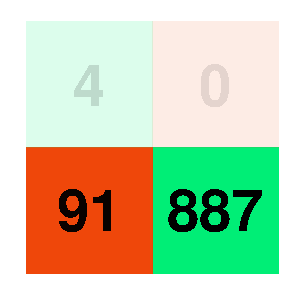
\includegraphics{Bank_Loan_Classification_files/figure-latex/unnamed-chunk-29-1.pdf}

Accuracy: 90.7331976\\
F1-Score: 0.0808081

\textbf{Linear Discriminant Analysis}

\begin{Shaded}
\begin{Highlighting}[]
\CommentTok{##---------Linear Discriminant Analysis------------##}
\CommentTok{# train}
\NormalTok{ld <-}\StringTok{ }\KeywordTok{train}\NormalTok{(personal_loan }\OperatorTok{~}\StringTok{ }\NormalTok{., }\DataTypeTok{data =}\NormalTok{ train, }\DataTypeTok{method =} \StringTok{"lda"}\NormalTok{, }\DataTypeTok{family =}\NormalTok{ binomial)}

\CommentTok{# predictions}
\NormalTok{pred_ld <-}\StringTok{ }\KeywordTok{predict}\NormalTok{(ld, val)}

\CommentTok{# Accuracy of the model}
\NormalTok{(acc_ld <-}\StringTok{ }\KeywordTok{mean}\NormalTok{(pred_ld }\OperatorTok{==}\StringTok{ }\NormalTok{val}\OperatorTok{$}\NormalTok{personal_loan))}
\end{Highlighting}
\end{Shaded}

\begin{verbatim}
## [1] 0.9480652
\end{verbatim}

\begin{Shaded}
\begin{Highlighting}[]
\CommentTok{# Generate Confusion Matrix of the model}
\NormalTok{results_ld <-}\StringTok{ }\KeywordTok{confusionMatrix}\NormalTok{(pred_ld, val}\OperatorTok{$}\NormalTok{personal_loan, }\DataTypeTok{positive=}\StringTok{"1"}\NormalTok{)}

\CommentTok{# F1 Score}
\NormalTok{(f1_ld <-}\StringTok{ }\NormalTok{results_ld}\OperatorTok{$}\NormalTok{byClass[}\StringTok{'F1'}\NormalTok{])}
\end{Highlighting}
\end{Shaded}

\begin{verbatim}
##        F1 
## 0.6982249
\end{verbatim}

\begin{Shaded}
\begin{Highlighting}[]
\CommentTok{# Draw a pretty confusion matrix using the custom helper function}
\KeywordTok{prettyConfusion}\NormalTok{(results_ld)}
\end{Highlighting}
\end{Shaded}

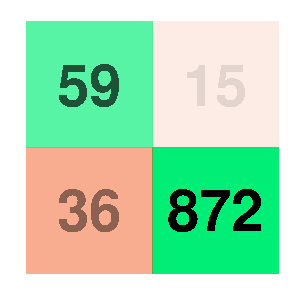
\includegraphics{Bank_Loan_Classification_files/figure-latex/unnamed-chunk-30-1.pdf}

Accuracy: 94.8065173\\
F1-Score: 0.6982249

\textbf{Loess}

\begin{Shaded}
\begin{Highlighting}[]
\CommentTok{##----------------------Loess--------------------##}

\CommentTok{# train}
\NormalTok{loess <-}\StringTok{ }\KeywordTok{train}\NormalTok{(personal_loan }\OperatorTok{~}\StringTok{ }\NormalTok{., }\DataTypeTok{data =}\NormalTok{ train, }\DataTypeTok{method =} \StringTok{"gamLoess"}\NormalTok{)}
\end{Highlighting}
\end{Shaded}

\begin{verbatim}
## Loading required package: gam
\end{verbatim}

\begin{verbatim}
## Loading required package: splines
\end{verbatim}

\begin{verbatim}
## Loading required package: foreach
\end{verbatim}

\begin{verbatim}
## 
## Attaching package: 'foreach'
\end{verbatim}

\begin{verbatim}
## The following objects are masked from 'package:purrr':
## 
##     accumulate, when
\end{verbatim}

\begin{verbatim}
## Loaded gam 1.16.1
\end{verbatim}

\begin{Shaded}
\begin{Highlighting}[]
\CommentTok{# predictions}
\NormalTok{pred_loess <-}\StringTok{ }\KeywordTok{predict}\NormalTok{(loess, val)}

\CommentTok{# Accuracy of the model}
\NormalTok{(acc_loess <-}\StringTok{ }\KeywordTok{mean}\NormalTok{(pred_loess }\OperatorTok{==}\StringTok{ }\NormalTok{val}\OperatorTok{$}\NormalTok{personal_loan))}
\end{Highlighting}
\end{Shaded}

\begin{verbatim}
## [1] 0.9765784
\end{verbatim}

\begin{Shaded}
\begin{Highlighting}[]
\CommentTok{# Generate Confusion Matrix of the model}
\NormalTok{results_loess <-}\StringTok{ }\KeywordTok{confusionMatrix}\NormalTok{(pred_loess, val}\OperatorTok{$}\NormalTok{personal_loan, }\DataTypeTok{positive=}\StringTok{"1"}\NormalTok{)}

\CommentTok{# F1 Score}
\NormalTok{(f1_loess <-}\StringTok{ }\NormalTok{results_loess}\OperatorTok{$}\NormalTok{byClass[}\StringTok{'F1'}\NormalTok{])}
\end{Highlighting}
\end{Shaded}

\begin{verbatim}
##        F1 
## 0.8715084
\end{verbatim}

\begin{Shaded}
\begin{Highlighting}[]
\CommentTok{# Draw a pretty confusion matrix using the custom helper function}
\KeywordTok{prettyConfusion}\NormalTok{(results_loess)}
\end{Highlighting}
\end{Shaded}

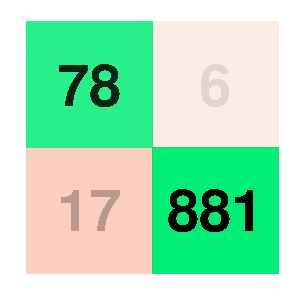
\includegraphics{Bank_Loan_Classification_files/figure-latex/unnamed-chunk-31-1.pdf}

Accuracy: 97.6578411\\
F1-Score: 0.8715084

\textbf{Quadratic Discriminant Analysis}

\begin{Shaded}
\begin{Highlighting}[]
\CommentTok{##--------Quadratic Discriminant Analysis----------##}

\CommentTok{# train}
\NormalTok{qd <-}\StringTok{ }\KeywordTok{train}\NormalTok{(personal_loan }\OperatorTok{~}\StringTok{ }\NormalTok{., }\DataTypeTok{data =}\NormalTok{ train, }\DataTypeTok{method =} \StringTok{"qda"}\NormalTok{, }\DataTypeTok{family =}\NormalTok{ binomial)}

\CommentTok{# predictions}
\NormalTok{pred_qd <-}\StringTok{ }\KeywordTok{predict}\NormalTok{(qd, val)}

\CommentTok{# Accuracy of the model}
\NormalTok{(acc_qd <-}\StringTok{ }\KeywordTok{mean}\NormalTok{(pred_qd }\OperatorTok{==}\StringTok{ }\NormalTok{val}\OperatorTok{$}\NormalTok{personal_loan))}
\end{Highlighting}
\end{Shaded}

\begin{verbatim}
## [1] 0.9429735
\end{verbatim}

\begin{Shaded}
\begin{Highlighting}[]
\CommentTok{# Generate Confusion Matrix of the model}
\NormalTok{results_qd <-}\StringTok{ }\KeywordTok{confusionMatrix}\NormalTok{(pred_qd, val}\OperatorTok{$}\NormalTok{personal_loan, }\DataTypeTok{positive=}\StringTok{"1"}\NormalTok{)}

\CommentTok{# F1 Score}
\NormalTok{(f1_qd <-}\StringTok{ }\NormalTok{results_qd}\OperatorTok{$}\NormalTok{byClass[}\StringTok{'F1'}\NormalTok{])}
\end{Highlighting}
\end{Shaded}

\begin{verbatim}
##        F1 
## 0.6818182
\end{verbatim}

\begin{Shaded}
\begin{Highlighting}[]
\CommentTok{# Draw a pretty confusion matrix using the custom helper function}
\KeywordTok{prettyConfusion}\NormalTok{(results_qd)}
\end{Highlighting}
\end{Shaded}

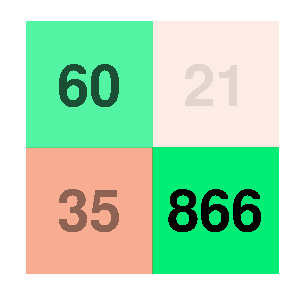
\includegraphics{Bank_Loan_Classification_files/figure-latex/unnamed-chunk-32-1.pdf}

Accuracy: 94.2973523\\
F1-Score: 0.6818182

\textbf{Support Vector Machine}

\begin{Shaded}
\begin{Highlighting}[]
\CommentTok{##----------Support Vector Machine----------------##}

\CommentTok{# train}
\NormalTok{svm <-}\StringTok{ }\KeywordTok{train}\NormalTok{(personal_loan }\OperatorTok{~}\StringTok{ }\NormalTok{., }\DataTypeTok{data =}\NormalTok{ train, }\DataTypeTok{method =} \StringTok{"svmLinear"}\NormalTok{)}

\CommentTok{# predictions}
\NormalTok{pred_svm <-}\StringTok{ }\KeywordTok{predict}\NormalTok{(loess, val)}

\CommentTok{# Accuracy of the model}
\NormalTok{(acc_svm <-}\StringTok{ }\KeywordTok{mean}\NormalTok{(pred_svm }\OperatorTok{==}\StringTok{ }\NormalTok{val}\OperatorTok{$}\NormalTok{personal_loan))}
\end{Highlighting}
\end{Shaded}

\begin{verbatim}
## [1] 0.9765784
\end{verbatim}

\begin{Shaded}
\begin{Highlighting}[]
\CommentTok{# Generate Confusion Matrix of the model}
\NormalTok{results_svm <-}\StringTok{ }\KeywordTok{confusionMatrix}\NormalTok{(pred_svm, val}\OperatorTok{$}\NormalTok{personal_loan, }\DataTypeTok{positive=}\StringTok{"1"}\NormalTok{)}

\CommentTok{# F1 Score}
\NormalTok{(f1_svm <-}\StringTok{ }\NormalTok{results_svm}\OperatorTok{$}\NormalTok{byClass[}\StringTok{'F1'}\NormalTok{])}
\end{Highlighting}
\end{Shaded}

\begin{verbatim}
##        F1 
## 0.8715084
\end{verbatim}

\begin{Shaded}
\begin{Highlighting}[]
\CommentTok{# Draw a pretty confusion matrix using the custom helper function}
\KeywordTok{prettyConfusion}\NormalTok{(results_svm)}
\end{Highlighting}
\end{Shaded}

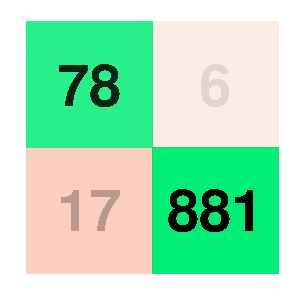
\includegraphics{Bank_Loan_Classification_files/figure-latex/unnamed-chunk-33-1.pdf}

Accuracy: 97.6578411\\
F1-Score: 0.8715084

\textbf{K Nearest Neighbours Classification}

\begin{Shaded}
\begin{Highlighting}[]
\CommentTok{##--------------K Nearest Neighbours--------------##}

\CommentTok{# Setting seed for reproducibility of results}
\KeywordTok{set.seed}\NormalTok{(}\DecValTok{7}\NormalTok{, }\DataTypeTok{sample.kind =} \StringTok{"Rounding"}\NormalTok{)}

\CommentTok{# k values to test best k}
\NormalTok{k_values <-}\StringTok{ }\KeywordTok{data.frame}\NormalTok{(}\DataTypeTok{k =} \KeywordTok{seq}\NormalTok{(}\DecValTok{2}\NormalTok{, }\DecValTok{12}\NormalTok{, }\DecValTok{1}\NormalTok{))}

\CommentTok{# train}
\NormalTok{knn <-}\StringTok{ }\KeywordTok{train}\NormalTok{(personal_loan }\OperatorTok{~}\StringTok{ }\NormalTok{., }\DataTypeTok{data =}\NormalTok{ train, }\DataTypeTok{method =} \StringTok{"knn"}\NormalTok{, }
             \DataTypeTok{tuneGrid =}\NormalTok{ k_values)}
\CommentTok{# best k value}
\NormalTok{knn}\OperatorTok{$}\NormalTok{bestTune}
\end{Highlighting}
\end{Shaded}

\begin{verbatim}
##   k
## 1 2
\end{verbatim}

\begin{Shaded}
\begin{Highlighting}[]
\CommentTok{# predictions}
\NormalTok{pred_knn <-}\StringTok{ }\KeywordTok{predict}\NormalTok{(knn, val)}

\CommentTok{# Accuracy of the model}
\NormalTok{(acc_knn <-}\StringTok{ }\KeywordTok{mean}\NormalTok{(pred_knn }\OperatorTok{==}\StringTok{ }\NormalTok{val}\OperatorTok{$}\NormalTok{personal_loan))}
\end{Highlighting}
\end{Shaded}

\begin{verbatim}
## [1] 0.9368635
\end{verbatim}

\begin{Shaded}
\begin{Highlighting}[]
\CommentTok{# Generate Confusion Matrix of the model}
\NormalTok{results_knn <-}\StringTok{ }\KeywordTok{confusionMatrix}\NormalTok{(pred_knn, val}\OperatorTok{$}\NormalTok{personal_loan, }\DataTypeTok{positive=}\StringTok{"1"}\NormalTok{)}

\CommentTok{# F1 Score}
\NormalTok{(f1_knn <-}\StringTok{ }\NormalTok{results_knn}\OperatorTok{$}\NormalTok{byClass[}\StringTok{'F1'}\NormalTok{])}
\end{Highlighting}
\end{Shaded}

\begin{verbatim}
##        F1 
## 0.5974026
\end{verbatim}

\begin{Shaded}
\begin{Highlighting}[]
\CommentTok{# Draw a pretty confusion matrix using the custom helper function}
\KeywordTok{prettyConfusion}\NormalTok{(results_knn)}
\end{Highlighting}
\end{Shaded}

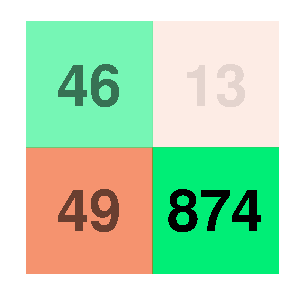
\includegraphics{Bank_Loan_Classification_files/figure-latex/unnamed-chunk-34-1.pdf}

The best k value is: 2\\
Accuracy: 93.6863544\\
F1-Score: 0.5974026

\textbf{Random Forest Classification}

\begin{Shaded}
\begin{Highlighting}[]
\CommentTok{##----------------Random Forest------------------##}

\CommentTok{# Setting seed for reproducibility of results}
\KeywordTok{set.seed}\NormalTok{(}\DecValTok{7}\NormalTok{, }\DataTypeTok{sample.kind =} \StringTok{"Rounding"}\NormalTok{)}

\CommentTok{# Values of mtry}
\NormalTok{mtryGrid <-}\StringTok{ }\KeywordTok{data.frame}\NormalTok{(}\DataTypeTok{mtry =} \KeywordTok{c}\NormalTok{(}\DecValTok{3}\NormalTok{,}\DecValTok{5}\NormalTok{,}\DecValTok{7}\NormalTok{,}\DecValTok{9}\NormalTok{))}

\CommentTok{# train}
\NormalTok{rf <-}\StringTok{  }\KeywordTok{train}\NormalTok{(personal_loan }\OperatorTok{~}\StringTok{ }\NormalTok{., }\DataTypeTok{data =}\NormalTok{ train, }\DataTypeTok{method =} \StringTok{"rf"}\NormalTok{,}
             \DataTypeTok{tuneGrid =}\NormalTok{ mtryGrid, }\DataTypeTok{importance =}\NormalTok{ T)}

\CommentTok{# Plot the values of accuracy for values of mtry}
\KeywordTok{ggplot}\NormalTok{(rf) }\OperatorTok{+}\StringTok{ }\KeywordTok{theme_minimal}\NormalTok{()}
\end{Highlighting}
\end{Shaded}

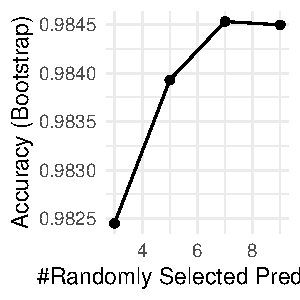
\includegraphics{Bank_Loan_Classification_files/figure-latex/unnamed-chunk-35-1.pdf}

\begin{Shaded}
\begin{Highlighting}[]
\CommentTok{# best model param}
\NormalTok{rf}\OperatorTok{$}\NormalTok{bestTune}
\end{Highlighting}
\end{Shaded}

\begin{verbatim}
##   mtry
## 3    7
\end{verbatim}

\begin{Shaded}
\begin{Highlighting}[]
\CommentTok{# predictions}
\NormalTok{pred_rf <-}\StringTok{ }\KeywordTok{predict}\NormalTok{(rf, val)}

\CommentTok{# Accuracy of the model}
\NormalTok{(acc_rf <-}\StringTok{ }\KeywordTok{mean}\NormalTok{(pred_rf }\OperatorTok{==}\StringTok{ }\NormalTok{val}\OperatorTok{$}\NormalTok{personal_loan))}
\end{Highlighting}
\end{Shaded}

\begin{verbatim}
## [1] 0.9898167
\end{verbatim}

\begin{Shaded}
\begin{Highlighting}[]
\CommentTok{# Generate Confusion Matrix of the model}
\NormalTok{results_rf <-}\StringTok{ }\KeywordTok{confusionMatrix}\NormalTok{(pred_rf, val}\OperatorTok{$}\NormalTok{personal_loan, }\DataTypeTok{positive=}\StringTok{"1"}\NormalTok{)}

\CommentTok{# F1 Score}
\NormalTok{(f1_rf <-}\StringTok{ }\NormalTok{results_rf}\OperatorTok{$}\NormalTok{byClass[}\StringTok{'F1'}\NormalTok{])}
\end{Highlighting}
\end{Shaded}

\begin{verbatim}
##        F1 
## 0.9456522
\end{verbatim}

\begin{Shaded}
\begin{Highlighting}[]
\CommentTok{# Draw a pretty confusion matrix using the custom helper function}
\KeywordTok{prettyConfusion}\NormalTok{(results_rf)}
\end{Highlighting}
\end{Shaded}

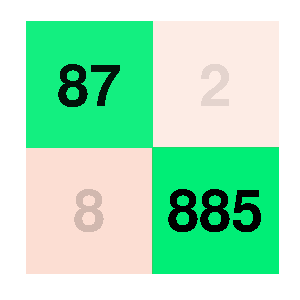
\includegraphics{Bank_Loan_Classification_files/figure-latex/unnamed-chunk-35-2.pdf}

The best value of mtry is: 7

Accuracy: 98.9816701\\
F1-Score: 0.9456522

\begin{Shaded}
\begin{Highlighting}[]
\CommentTok{#Variable Importance}
\KeywordTok{varImp}\NormalTok{(rf)}
\end{Highlighting}
\end{Shaded}

\begin{verbatim}
## rf variable importance
## 
##                     Importance
## income                 100.000
## education3              69.072
## education2              63.508
## family4                 39.166
## family3                 38.807
## credit_card_spend       19.727
## family2                  6.986
## age                      5.080
## cd_account1              3.538
## credit_card1             1.847
## online1                  1.454
## mortgage                 1.002
## securities_account1      0.000
\end{verbatim}

We note that income, family and credit card are most important
variables. This was also confirmed in our exploratory data analysis
section.

\textbf{Ensemble Model (Voting Classifier)}

\begin{Shaded}
\begin{Highlighting}[]
\CommentTok{# votes are added up as total predictions from 6models that predict 1}
\NormalTok{votes <-}\StringTok{ }\NormalTok{(pred_rf }\OperatorTok{==}\StringTok{ }\DecValTok{1}\NormalTok{) }\OperatorTok{+}\StringTok{ }\NormalTok{(pred_svm }\OperatorTok{==}\StringTok{ }\DecValTok{1}\NormalTok{) }\OperatorTok{+}\StringTok{ }\NormalTok{(pred_ld }\OperatorTok{==}\StringTok{ }\DecValTok{1}\NormalTok{) }\OperatorTok{+}\StringTok{ }\NormalTok{(pred_lr }\OperatorTok{==}\StringTok{ }\DecValTok{1}\NormalTok{) }\OperatorTok{+}\StringTok{ }\NormalTok{(pred_loess }\OperatorTok{==}\StringTok{ }\DecValTok{1}\NormalTok{)}

\CommentTok{# Ensemble prediction is 1 if atleast three of the five models predict 1}
\NormalTok{pred_ensemble <-}\StringTok{ }\KeywordTok{ifelse}\NormalTok{(votes }\OperatorTok{>=}\StringTok{ }\DecValTok{3}\NormalTok{, }\DecValTok{1}\NormalTok{, }\DecValTok{0}\NormalTok{)}

\CommentTok{# Accuradcy of the model}
\NormalTok{(acc_ensemble <-}\StringTok{ }\KeywordTok{mean}\NormalTok{(pred_ensemble }\OperatorTok{==}\StringTok{ }\NormalTok{val}\OperatorTok{$}\NormalTok{personal_loan))}
\end{Highlighting}
\end{Shaded}

\begin{verbatim}
## [1] 0.9786151
\end{verbatim}

\begin{Shaded}
\begin{Highlighting}[]
\CommentTok{# Generate Confusion Matrix of the model}
\NormalTok{results_ensemble <-}\StringTok{ }\KeywordTok{confusionMatrix}\NormalTok{(}\KeywordTok{factor}\NormalTok{(pred_ensemble), val}\OperatorTok{$}\NormalTok{personal_loan, }\DataTypeTok{positive=}\StringTok{"1"}\NormalTok{)}

\CommentTok{# F1 Score}
\NormalTok{(f1_ensemble <-}\StringTok{ }\NormalTok{results_ensemble}\OperatorTok{$}\NormalTok{byClass[}\StringTok{'F1'}\NormalTok{])}
\end{Highlighting}
\end{Shaded}

\begin{verbatim}
##   F1 
## 0.88
\end{verbatim}

\begin{Shaded}
\begin{Highlighting}[]
\CommentTok{# Draw a pretty confusion matrix using the custom helper function}
\KeywordTok{prettyConfusion}\NormalTok{(results_ensemble)}
\end{Highlighting}
\end{Shaded}

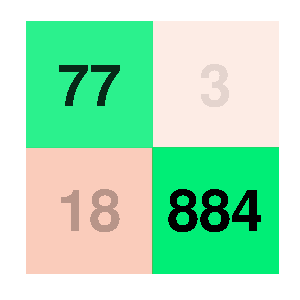
\includegraphics{Bank_Loan_Classification_files/figure-latex/unnamed-chunk-37-1.pdf}

Accuracy: 97.8615071\\
F1-Score: 0.88

\pagebreak

\hypertarget{validation-metrics}{%
\subsection{Validation Metrics}\label{validation-metrics}}

\hypertarget{validation-accuracies}{%
\subsubsection{Validation Accuracies}\label{validation-accuracies}}

\begin{Shaded}
\begin{Highlighting}[]
\CommentTok{#All models Validation Accuracies}
\NormalTok{models <-}\StringTok{ }\KeywordTok{c}\NormalTok{(}\StringTok{"Logistic regression"}\NormalTok{, }\StringTok{"Naive Bayes Classifier"}\NormalTok{,}
            \StringTok{"LDA"}\NormalTok{, }\StringTok{"QDA"}\NormalTok{, }\StringTok{"Loess"}\NormalTok{,}\StringTok{"K nearest neighbors"}\NormalTok{,}
            \StringTok{"Random forest"}\NormalTok{, }\StringTok{"Ensemble"}\NormalTok{ , }\StringTok{"Support Vector Machine"}\NormalTok{)}
\CommentTok{# Accuracy list}
\NormalTok{accuracy <-}\StringTok{ }\KeywordTok{c}\NormalTok{(acc_lr, acc_nb, acc_ld, acc_qd, acc_loess, acc_knn, acc_rf, acc_ensemble, acc_svm)}

\CommentTok{# Output the accuracies table}
\KeywordTok{data.frame}\NormalTok{(}\DataTypeTok{Model =}\NormalTok{ models, }\DataTypeTok{Validation_Accuracy =}\NormalTok{ accuracy) }\OperatorTok
\StringTok{  }\KeywordTok{arrange}\NormalTok{(}\KeywordTok{desc}\NormalTok{(Validation_Accuracy)) }\OperatorTok
\StringTok{  }\NormalTok{knitr}\OperatorTok{::}\KeywordTok{kable}\NormalTok{()}
\end{Highlighting}
\end{Shaded}

\begin{longtable}[]{@{}lr@{}}
\toprule
Model & Validation\_Accuracy\tabularnewline
\midrule
\endhead
Random forest & 0.9898167\tabularnewline
Ensemble & 0.9786151\tabularnewline
Loess & 0.9765784\tabularnewline
Support Vector Machine & 0.9765784\tabularnewline
Logistic regression & 0.9602851\tabularnewline
LDA & 0.9480652\tabularnewline
QDA & 0.9429735\tabularnewline
K nearest neighbors & 0.9368635\tabularnewline
Naive Bayes Classifier & 0.9073320\tabularnewline
\bottomrule
\end{longtable}

\hypertarget{validation-f1-scores}{%
\subsubsection{Validation F1-Scores}\label{validation-f1-scores}}

\begin{Shaded}
\begin{Highlighting}[]
\CommentTok{# All models Validation F1 Scores}
\NormalTok{f1 <-}\StringTok{ }\KeywordTok{c}\NormalTok{(f1_lr, f1_nb, f1_ld, f1_qd, f1_loess, f1_knn, f1_rf, f1_ensemble, f1_svm)}

\CommentTok{# Output the f1 table}
\KeywordTok{data.frame}\NormalTok{(}\DataTypeTok{Model =}\NormalTok{ models, }\DataTypeTok{Validation_F1 =}\NormalTok{ f1) }\OperatorTok
\StringTok{  }\KeywordTok{arrange}\NormalTok{(}\KeywordTok{desc}\NormalTok{(Validation_F1)) }\OperatorTok
\StringTok{  }\NormalTok{knitr}\OperatorTok{::}\KeywordTok{kable}\NormalTok{()}
\end{Highlighting}
\end{Shaded}

\begin{longtable}[]{@{}lr@{}}
\toprule
Model & Validation\_F1\tabularnewline
\midrule
\endhead
Random forest & 0.9456522\tabularnewline
Ensemble & 0.8800000\tabularnewline
Loess & 0.8715084\tabularnewline
Support Vector Machine & 0.8715084\tabularnewline
Logistic regression & 0.7719298\tabularnewline
LDA & 0.6982249\tabularnewline
QDA & 0.6818182\tabularnewline
K nearest neighbors & 0.5974026\tabularnewline
Naive Bayes Classifier & 0.0808081\tabularnewline
\pagebreak &\tabularnewline
\bottomrule
\end{longtable}

The best performing models on validation set are:

\begin{verbatim}
1. Random Forest
2. Ensemble Voting Classifier
3. Loess 
4. Support Vector Machine
5. Logistic Regression Classifier
6. Linear Discriminant Analysis 
\end{verbatim}

\hypertarget{model-evaluation}{%
\section{Model Evaluation}\label{model-evaluation}}

We generate the predictions for the test set using our best models
selected using validation F1-Scores:

\begin{Shaded}
\begin{Highlighting}[]
\CommentTok{# Logistic Regression test set predictions}
\NormalTok{test_lr <-}\StringTok{ }\KeywordTok{predict}\NormalTok{(lr, test)}

\CommentTok{# Confusion matrix for the test predictions of lr model}
\NormalTok{test_results_lr <-}\StringTok{ }\KeywordTok{confusionMatrix}\NormalTok{(test_lr, test}\OperatorTok{$}\NormalTok{personal_loan, }\DataTypeTok{positive=}\StringTok{"1"}\NormalTok{)}

\CommentTok{# F1 Score}
\NormalTok{(test_f1_lr <-}\StringTok{ }\NormalTok{test_results_lr}\OperatorTok{$}\NormalTok{byClass[}\StringTok{'F1'}\NormalTok{])}
\end{Highlighting}
\end{Shaded}

\begin{verbatim}
##        F1 
## 0.7816092
\end{verbatim}

\begin{Shaded}
\begin{Highlighting}[]
\CommentTok{# LDA test set predictions}
\NormalTok{test_ld <-}\StringTok{ }\KeywordTok{predict}\NormalTok{(ld, test)}

\CommentTok{# Confusion matrix for the test predictions of lda model}
\NormalTok{test_results_ld <-}\StringTok{ }\KeywordTok{confusionMatrix}\NormalTok{(test_ld, test}\OperatorTok{$}\NormalTok{personal_loan, }\DataTypeTok{positive=}\StringTok{"1"}\NormalTok{)}

\CommentTok{# F1 Score}
\NormalTok{(test_f1_ld <-}\StringTok{ }\NormalTok{test_results_ld}\OperatorTok{$}\NormalTok{byClass[}\StringTok{'F1'}\NormalTok{])}
\end{Highlighting}
\end{Shaded}

\begin{verbatim}
##        F1 
## 0.6936416
\end{verbatim}

\begin{Shaded}
\begin{Highlighting}[]
\CommentTok{# Loess test set predictions}
\NormalTok{test_loess <-}\StringTok{ }\KeywordTok{predict}\NormalTok{(loess, test)}

\CommentTok{# Confusion matrix for the test predictions of loess model}
\NormalTok{test_results_loess <-}\StringTok{ }\KeywordTok{confusionMatrix}\NormalTok{(test_loess, test}\OperatorTok{$}\NormalTok{personal_loan, }\DataTypeTok{positive=}\StringTok{"1"}\NormalTok{)}

\CommentTok{# F1 Score}
\NormalTok{(test_f1_loess <-}\StringTok{ }\NormalTok{test_results_loess}\OperatorTok{$}\NormalTok{byClass[}\StringTok{'F1'}\NormalTok{])}
\end{Highlighting}
\end{Shaded}

\begin{verbatim}
##        F1 
## 0.8342246
\end{verbatim}

\begin{Shaded}
\begin{Highlighting}[]
\CommentTok{# SVM test set predictions}
\NormalTok{test_svm <-}\StringTok{ }\KeywordTok{predict}\NormalTok{(svm, test)}

\CommentTok{# Confusion matrix for the test predictions of svm model}
\NormalTok{test_results_svm <-}\StringTok{ }\KeywordTok{confusionMatrix}\NormalTok{(test_svm, test}\OperatorTok{$}\NormalTok{personal_loan, }\DataTypeTok{positive=}\StringTok{"1"}\NormalTok{)}

\CommentTok{# F1 Score}
\NormalTok{(test_f1_svm <-}\StringTok{ }\NormalTok{test_results_svm}\OperatorTok{$}\NormalTok{byClass[}\StringTok{'F1'}\NormalTok{])}
\end{Highlighting}
\end{Shaded}

\begin{verbatim}
##        F1 
## 0.7664671
\end{verbatim}

\begin{Shaded}
\begin{Highlighting}[]
\CommentTok{# Random Forest test set predictions}
\NormalTok{test_rf <-}\StringTok{ }\KeywordTok{predict}\NormalTok{(rf, test)}

\CommentTok{# Confusion matrix for the test predictions of random forest model}
\NormalTok{test_results_rf <-}\StringTok{ }\KeywordTok{confusionMatrix}\NormalTok{(test_rf, test}\OperatorTok{$}\NormalTok{personal_loan, }\DataTypeTok{positive=}\StringTok{"1"}\NormalTok{)}

\CommentTok{# F1 Score}
\NormalTok{(test_f1_rf <-}\StringTok{ }\NormalTok{test_results_rf}\OperatorTok{$}\NormalTok{byClass[}\StringTok{'F1'}\NormalTok{])}
\end{Highlighting}
\end{Shaded}

\begin{verbatim}
##        F1 
## 0.9109948
\end{verbatim}

\begin{Shaded}
\begin{Highlighting}[]
\CommentTok{# votes are added up as total predictions from 6models that predict 1}
\NormalTok{test_votes <-}\StringTok{ }\NormalTok{(test_rf }\OperatorTok{==}\StringTok{ }\DecValTok{1}\NormalTok{) }\OperatorTok{+}\StringTok{ }\NormalTok{(test_loess }\OperatorTok{==}\StringTok{ }\DecValTok{1}\NormalTok{) }\OperatorTok{+}\StringTok{ }\NormalTok{(test_svm }\OperatorTok{==}\StringTok{ }\DecValTok{1}\NormalTok{) }\OperatorTok{+}\StringTok{ }\NormalTok{(test_lr }\OperatorTok{==}\StringTok{ }\DecValTok{1}\NormalTok{) }\OperatorTok{+}\StringTok{ }\NormalTok{(test_ld }\OperatorTok{==}\StringTok{ }\DecValTok{1}\NormalTok{)}

\CommentTok{# Ensemble test set predictions}
\NormalTok{test_ensemble <-}\StringTok{ }\KeywordTok{ifelse}\NormalTok{(test_votes }\OperatorTok{>=}\StringTok{ }\DecValTok{3}\NormalTok{, }\DecValTok{1}\NormalTok{, }\DecValTok{0}\NormalTok{)}

\CommentTok{# Confusion matrix for the test predictions of ensemble model}
\NormalTok{test_results_ensemble <-}\StringTok{ }\KeywordTok{confusionMatrix}\NormalTok{(}\KeywordTok{factor}\NormalTok{(test_ensemble), test}\OperatorTok{$}\NormalTok{personal_loan, }\DataTypeTok{positive=}\StringTok{"1"}\NormalTok{)}

\CommentTok{# F1 Score}
\NormalTok{(test_f1_ensemble <-}\StringTok{ }\NormalTok{test_results_ensemble}\OperatorTok{$}\NormalTok{byClass[}\StringTok{'F1'}\NormalTok{])}
\end{Highlighting}
\end{Shaded}

\begin{verbatim}
##        F1 
## 0.8023256
\end{verbatim}

\pagebreak

\hypertarget{results}{%
\section{Results}\label{results}}

Here we obatin the results for the best models on the test set as
follows:

\hypertarget{testing-accuracies}{%
\subsection{Testing Accuracies}\label{testing-accuracies}}

\begin{Shaded}
\begin{Highlighting}[]
\CommentTok{# Selected models}
\NormalTok{test_models <-}\StringTok{ }\KeywordTok{c}\NormalTok{(}\StringTok{"Random Forest"}\NormalTok{, }\StringTok{"Loess"}\NormalTok{ , }\StringTok{"Support Vector Machine"}\NormalTok{,}
                 \StringTok{"Logistic Regression"}\NormalTok{, }\StringTok{"Linear Discriminatn Analyis"}\NormalTok{, }\StringTok{"Ensemble"}\NormalTok{)}

\CommentTok{# Calculate Accuracies for the test set}
\NormalTok{test_accuracy <-}\StringTok{ }\KeywordTok{c}\NormalTok{(}\KeywordTok{mean}\NormalTok{(test_rf }\OperatorTok{==}\StringTok{ }\NormalTok{test}\OperatorTok{$}\NormalTok{personal_loan),}
                   \KeywordTok{mean}\NormalTok{(test_loess }\OperatorTok{==}\StringTok{ }\NormalTok{test}\OperatorTok{$}\NormalTok{personal_loan),}
                   \KeywordTok{mean}\NormalTok{(test_svm }\OperatorTok{==}\StringTok{ }\NormalTok{test}\OperatorTok{$}\NormalTok{personal_loan),}
                   \KeywordTok{mean}\NormalTok{(test_lr }\OperatorTok{==}\StringTok{ }\NormalTok{test}\OperatorTok{$}\NormalTok{personal_loan),}
                   \KeywordTok{mean}\NormalTok{(test_ld }\OperatorTok{==}\StringTok{ }\NormalTok{test}\OperatorTok{$}\NormalTok{personal_loan),}
                   \KeywordTok{mean}\NormalTok{(test_ensemble }\OperatorTok{==}\StringTok{ }\NormalTok{test}\OperatorTok{$}\NormalTok{personal_loan))}

\CommentTok{# Output the testing accuracies table}
\KeywordTok{data.frame}\NormalTok{(}\DataTypeTok{Model =}\NormalTok{ test_models, }\DataTypeTok{Testing_Accuracy =}\NormalTok{ test_accuracy) }\OperatorTok
\StringTok{  }\KeywordTok{arrange}\NormalTok{(}\KeywordTok{desc}\NormalTok{(Testing_Accuracy)) }\OperatorTok
\StringTok{  }\NormalTok{knitr}\OperatorTok{::}\KeywordTok{kable}\NormalTok{()}
\end{Highlighting}
\end{Shaded}

\begin{longtable}[]{@{}lr@{}}
\toprule
Model & Testing\_Accuracy\tabularnewline
\midrule
\endhead
Random Forest & 0.9831014\tabularnewline
Loess & 0.9691849\tabularnewline
Ensemble & 0.9662028\tabularnewline
Logistic Regression & 0.9622266\tabularnewline
Support Vector Machine & 0.9612326\tabularnewline
Linear Discriminatn Analyis & 0.9473161\tabularnewline
\bottomrule
\end{longtable}

\hypertarget{testing-f1-scores}{%
\subsection{Testing F1-Scores}\label{testing-f1-scores}}

\begin{Shaded}
\begin{Highlighting}[]
\CommentTok{# All models Validation F1 Scores}
\NormalTok{test_f1 <-}\StringTok{ }\KeywordTok{c}\NormalTok{(test_f1_rf, test_f1_loess, test_f1_svm, }
\NormalTok{             test_f1_lr, test_f1_ld, test_f1_ensemble)}

\CommentTok{# Output the f1 table}
\KeywordTok{data.frame}\NormalTok{(}\DataTypeTok{Model =}\NormalTok{ test_models, }\DataTypeTok{Testing_F1 =}\NormalTok{ test_f1) }\OperatorTok
\StringTok{  }\KeywordTok{arrange}\NormalTok{(}\KeywordTok{desc}\NormalTok{(Testing_F1)) }\OperatorTok
\StringTok{  }\NormalTok{knitr}\OperatorTok{::}\KeywordTok{kable}\NormalTok{()}
\end{Highlighting}
\end{Shaded}

\begin{longtable}[]{@{}lr@{}}
\toprule
Model & Testing\_F1\tabularnewline
\midrule
\endhead
Random Forest & 0.9109948\tabularnewline
Loess & 0.8342246\tabularnewline
Ensemble & 0.8023256\tabularnewline
Logistic Regression & 0.7816092\tabularnewline
Support Vector Machine & 0.7664671\tabularnewline
Linear Discriminatn Analyis & 0.6936416\tabularnewline
\bottomrule
\end{longtable}

\pagebreak

\hypertarget{conclusion}{%
\section{Conclusion}\label{conclusion}}

Finally, we conclude that the best model for this project was the random
forest model(7). It had a testing F1-Score of 0.911 and Testing Accuracy
98.31\%.\\
Further scope for this project would be to incorporate neural networks
and gradient boosting models which might improve on our models, however,
given the time taken to train and tune neural networks. We have left it
to the future. Also, we could do some feature engineering to find out
the main features and if possible, extract new features from the domain.

This analysis could've been better if we get more data from Bank of
India so that the we can be sure that the models are not over-fitting to
this specific dataset and generalize better to new or unseeen data.

\end{document}
